\import{appendices/}{manySubfigsChapterHeader}%
This appendix illustrates the use of the $\backslash$\texttt{ContinuedFloat} command (from the \texttt{subfig} package) to break a figure that includes several sub-figures (more than will fit on one page) into multiple figures.
Also, the \texttt{alphalph} package is used to handle the creation of letter labels for situations where more than 26 entities are labelled.
\autoref{fig:instructions1} is a figure with 28 subfigures.
Note that \autoref{subfig:instructionsExampleSuccess} is correctly labelled.

%% For this chapter, we did not define a rule (with \DeclareGraphicsRule)
%% telling LaTeX how to get the bounding box for raster image files.
%% Instead, we use the graphicx package's \setkeys command to define some
%% keys for all the figures included in this chapter:
\setkeys{Gin}{natwidth=1600px,natheight=1200px,width=13cm}%
\begin{figure}%
\centering%
\subfloat[][The background/text colours have been inverted for clarity in this medium.]{%
\label{subfig:instructionsPurpose}%
\fbox{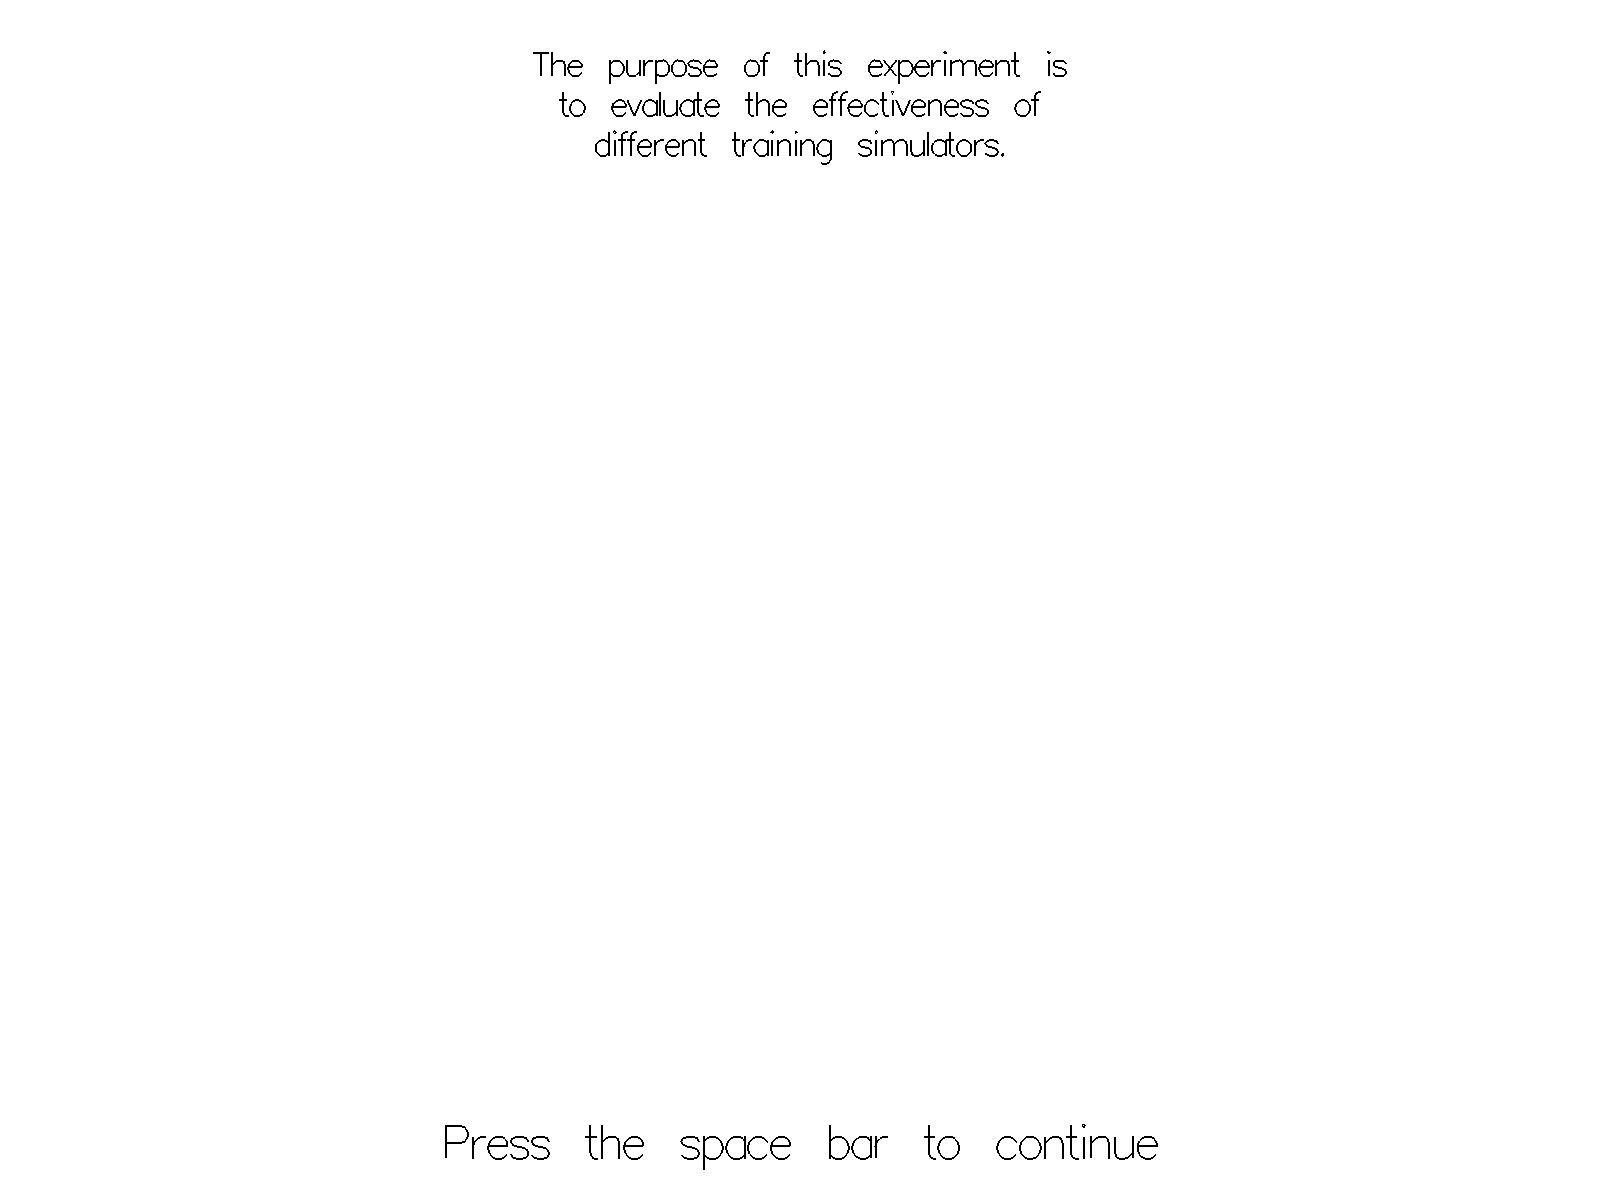
\includegraphics{figures/Purpose}}%
}%
\linebreak%
\subfloat[][]{%
\label{subfig:instructionsToday}%
\fbox{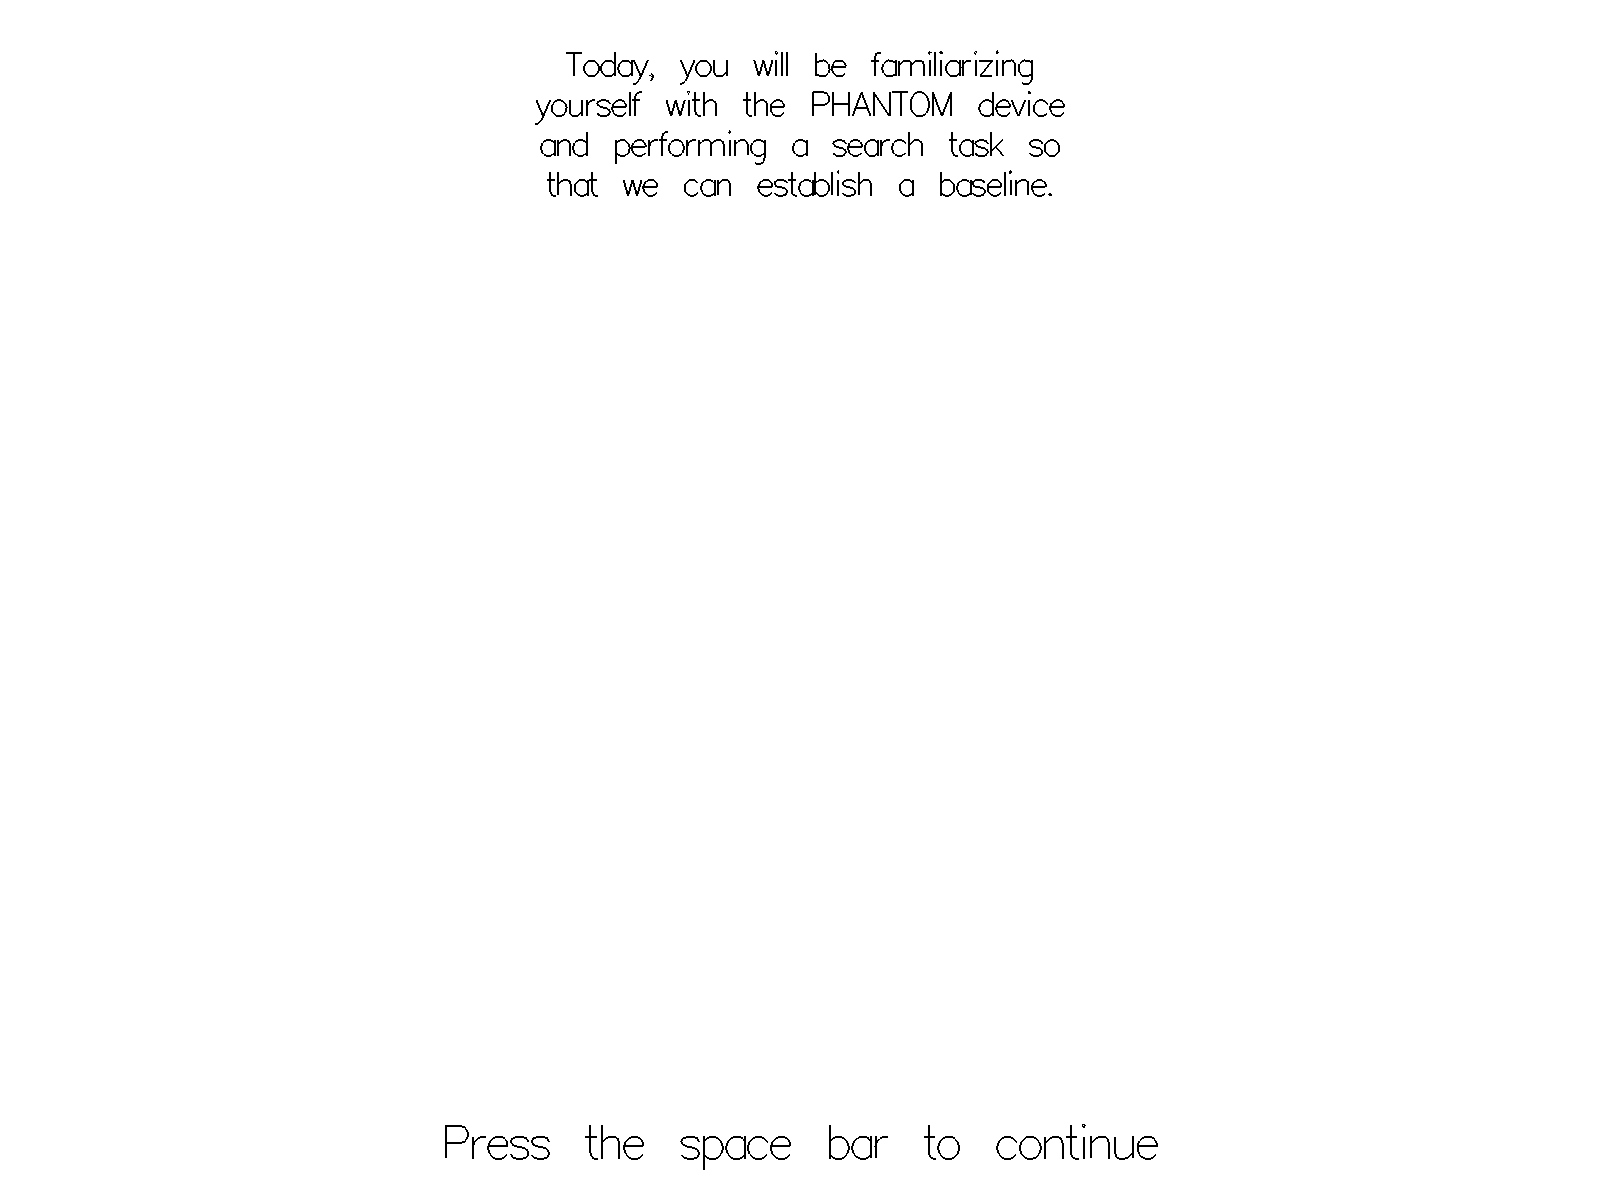
\includegraphics{figures/Today}}%
}%
\caption[User Study Instructions]{%
  Instructions presented to the subject (continued below).
}%
\label{fig:instructions1}%
\end{figure}%

\begin{figure}%
\ContinuedFloat%
\centering%
\subfloat[][]{%
\label{subfig:instructionsPhantom}%
\fbox{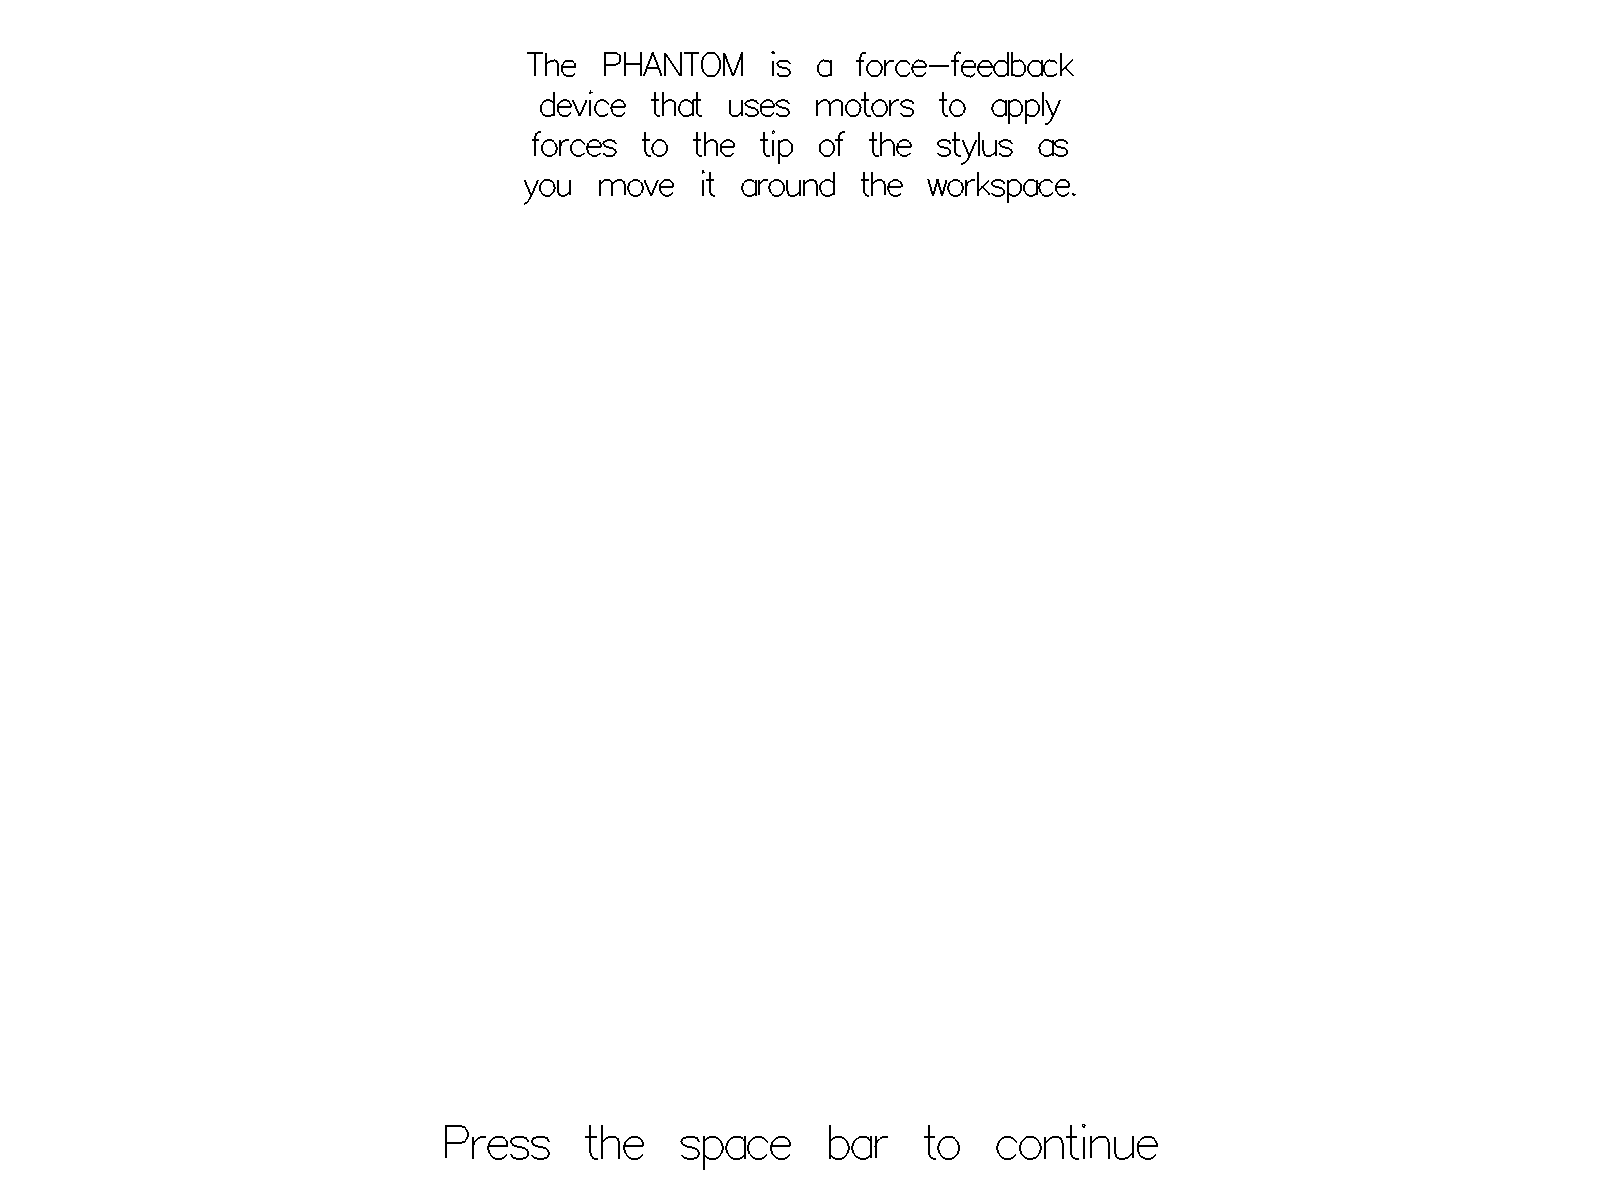
\includegraphics{figures/Phantom}}%
}%
\linebreak%
\subfloat[][The position of the haptic master within the workspace is indicated by the yellow sphere.]{%
\label{subfig:instructionsMotorsOff}%
\fbox{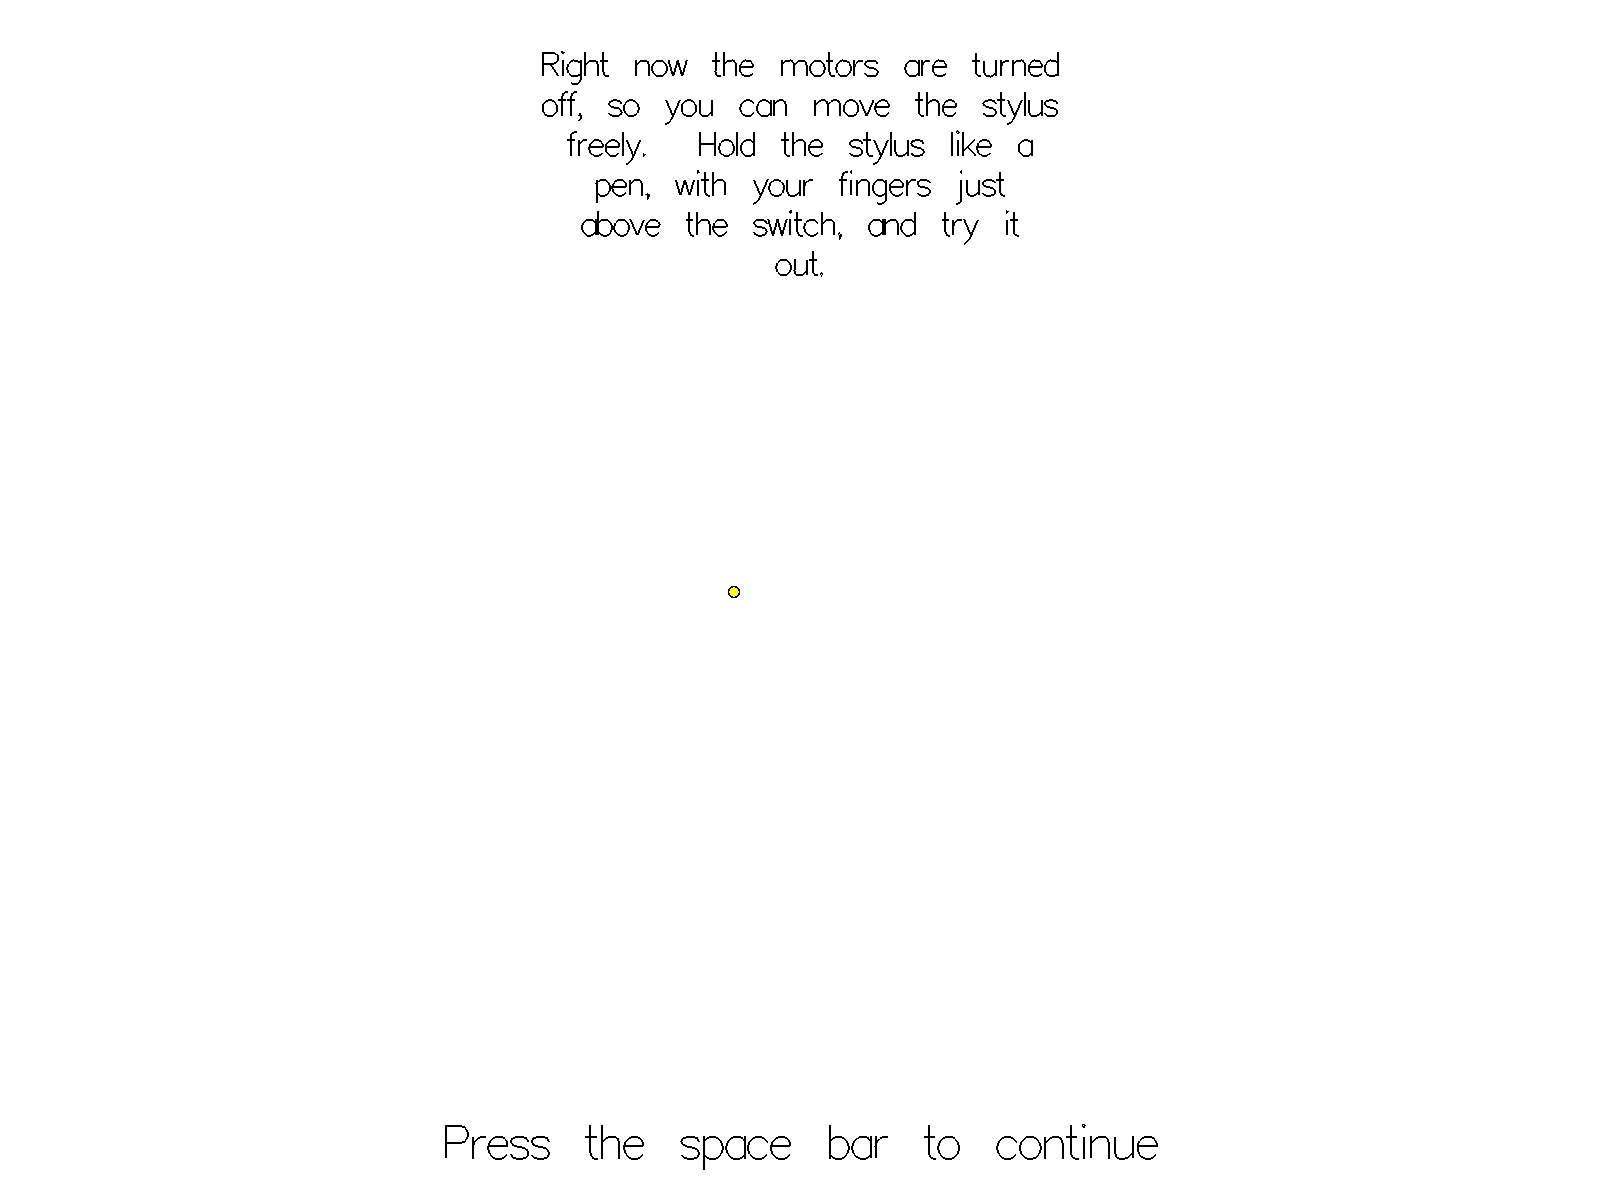
\includegraphics{figures/MotorsOff}}%
}%
\caption[]{}%
\label{fig:instructions2}%
\end{figure}%

\begin{figure}%
\ContinuedFloat%
\centering%
\subfloat[][]{%
\label{subfig:instructionsReadyToActivateSpring}%
\fbox{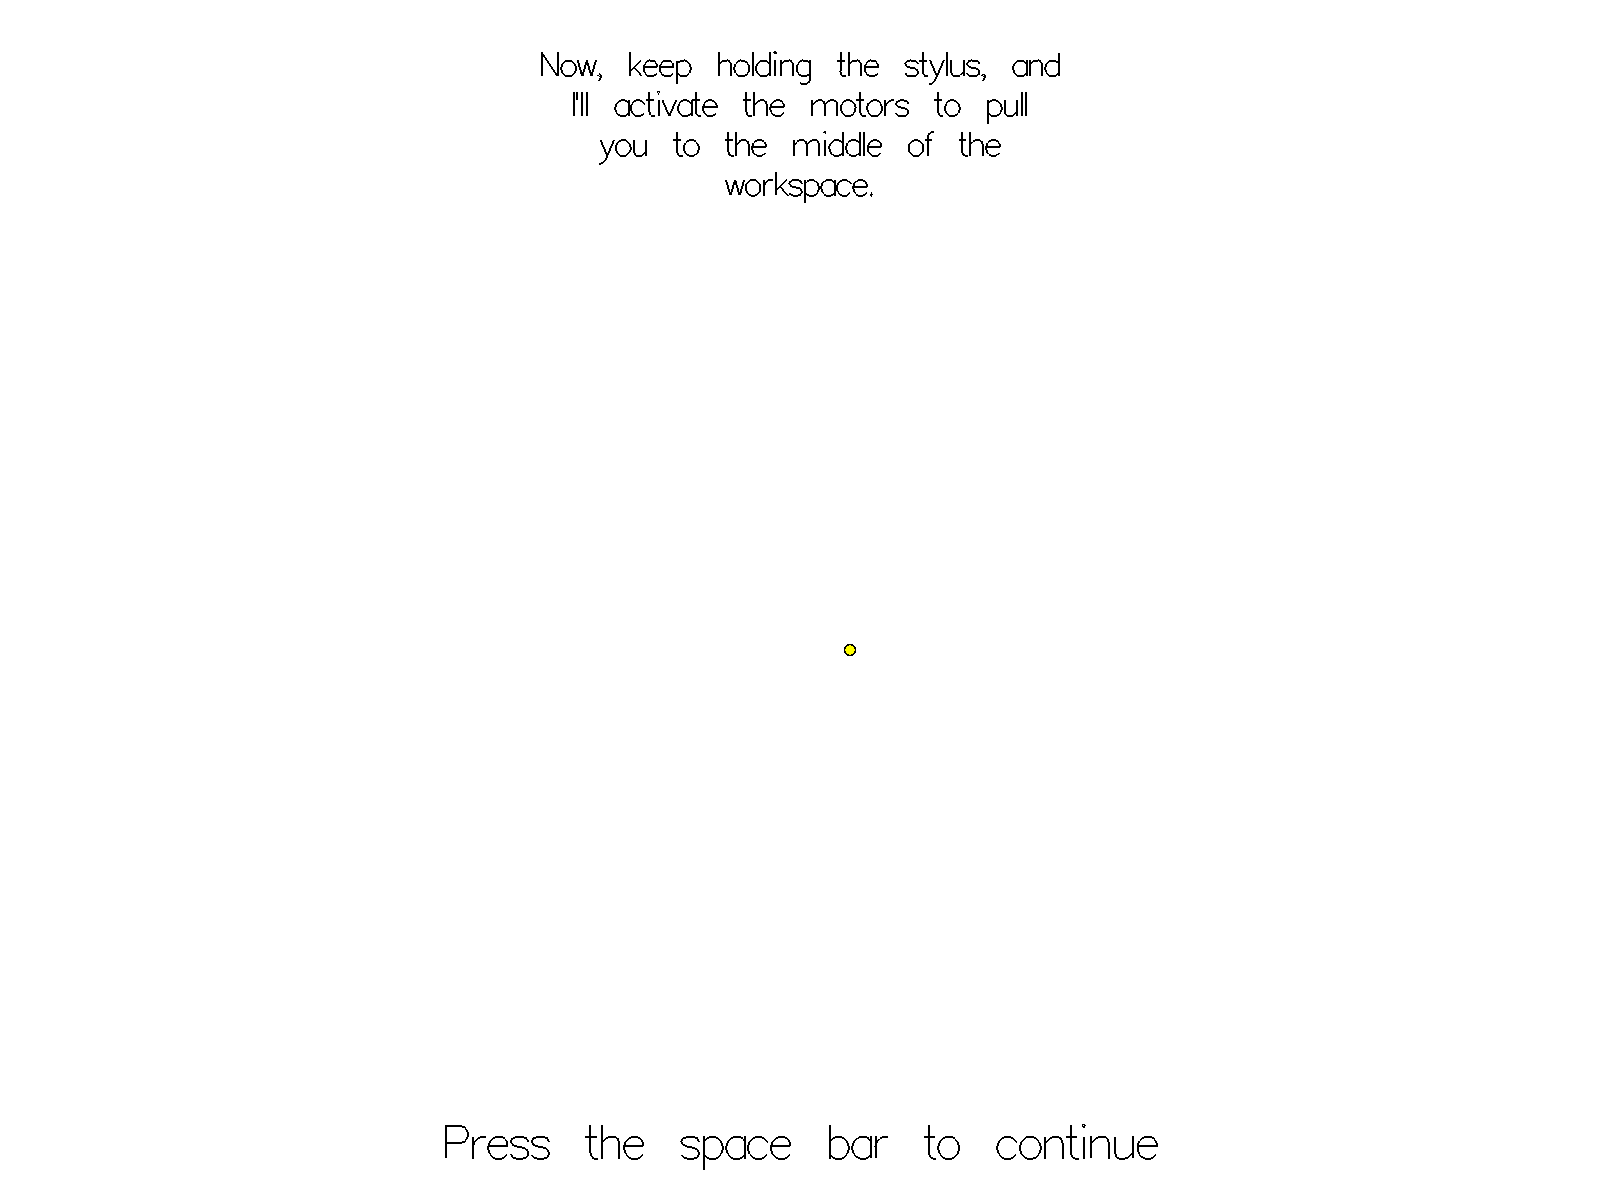
\includegraphics{figures/ReadyToActivateSpring}}%
}%
\linebreak%
\subfloat[][]{%
\label{subfig:instructionsSpringActive}%
\fbox{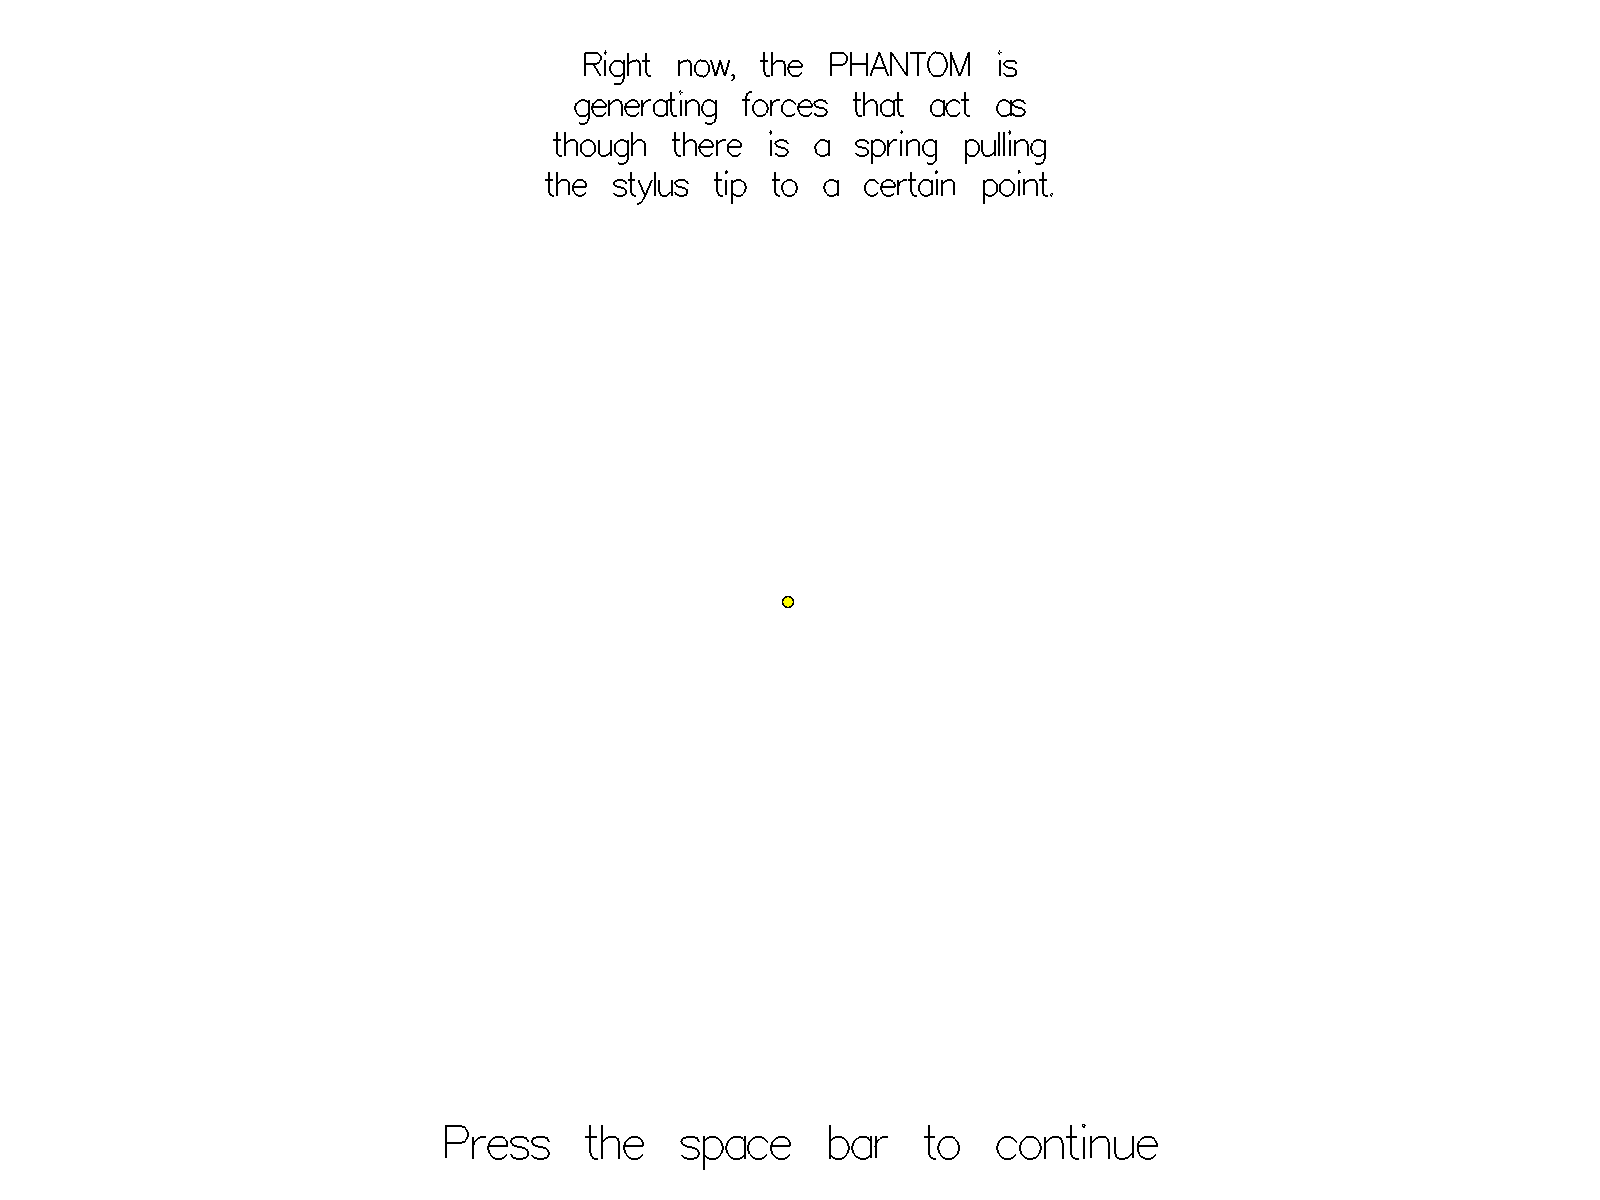
\includegraphics{figures/SpringActive}}%
}%
\caption[]{}%
\label{fig:instructions3}%
\end{figure}%

\begin{figure}%
\ContinuedFloat%
\centering%
\subfloat[][]{%
\label{subfig:instructionsReadyToDeactivateSpring}%
\fbox{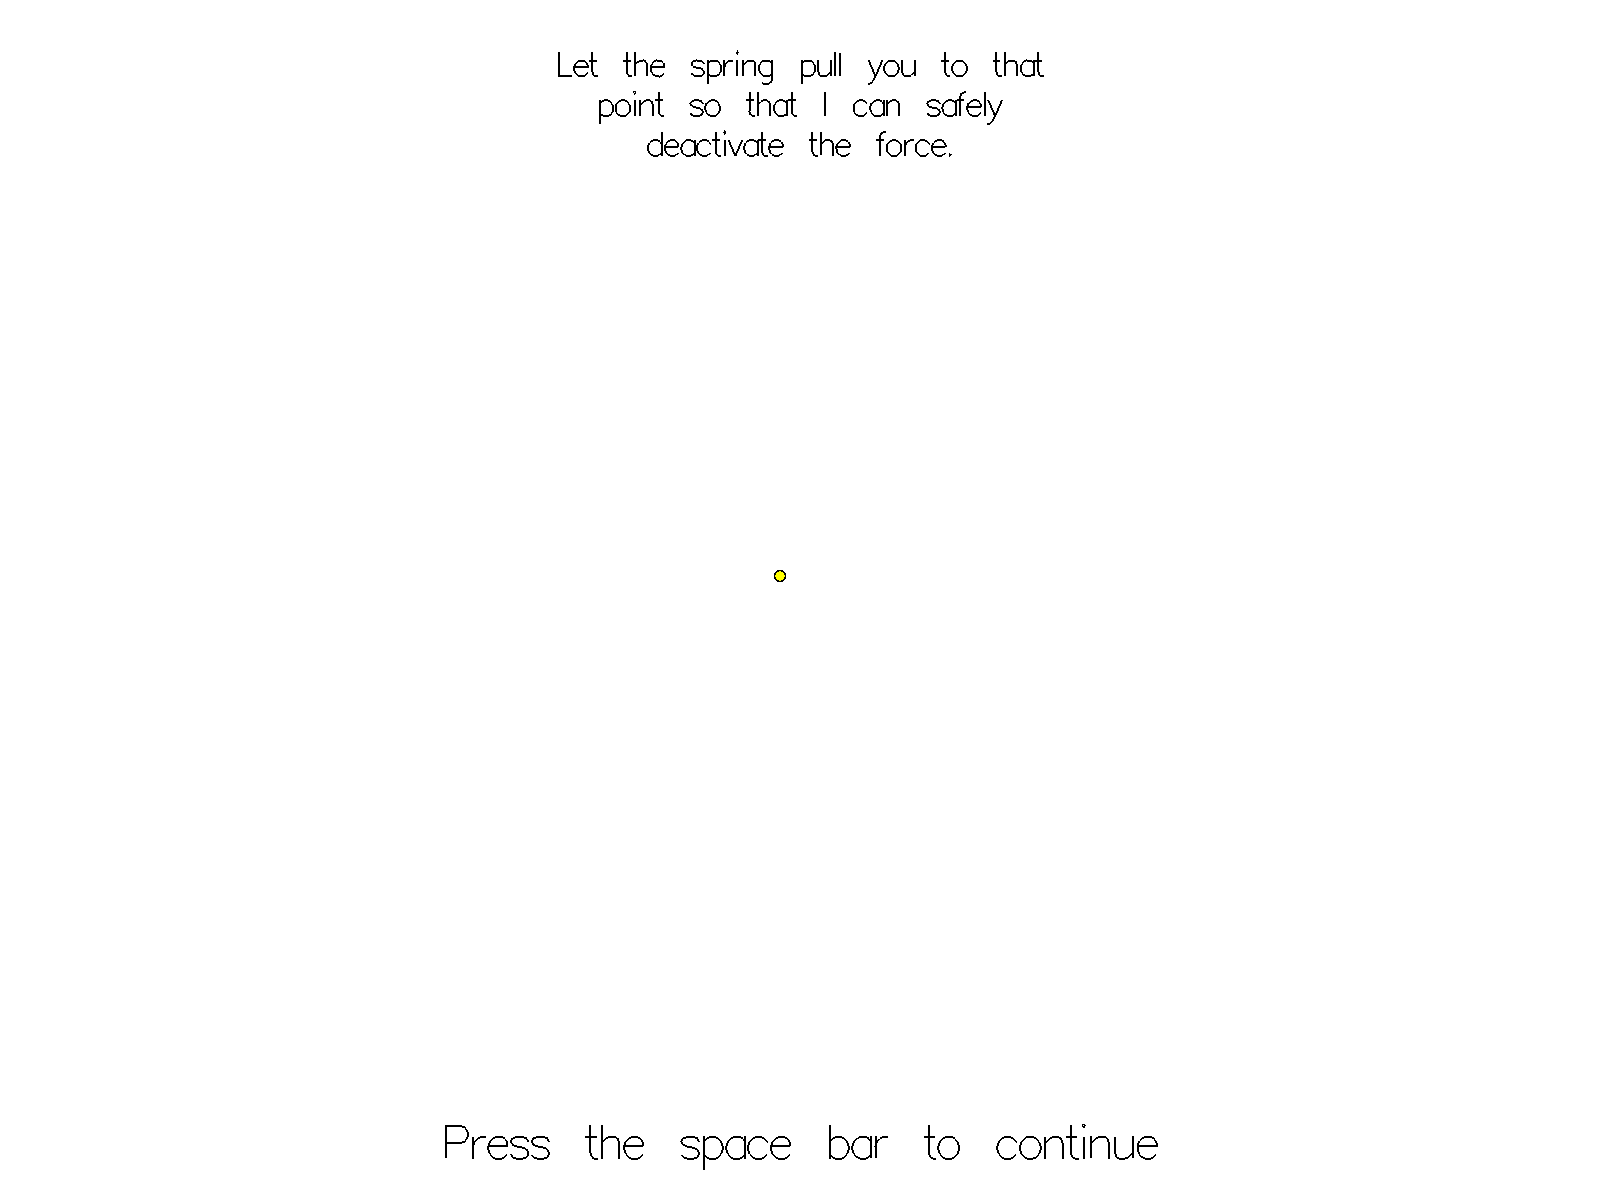
\includegraphics{figures/ReadyToDeactivateSpring}}%
}%
\linebreak%
\subfloat[][]{%
\label{subfig:instructionsSolidSurface}%
\fbox{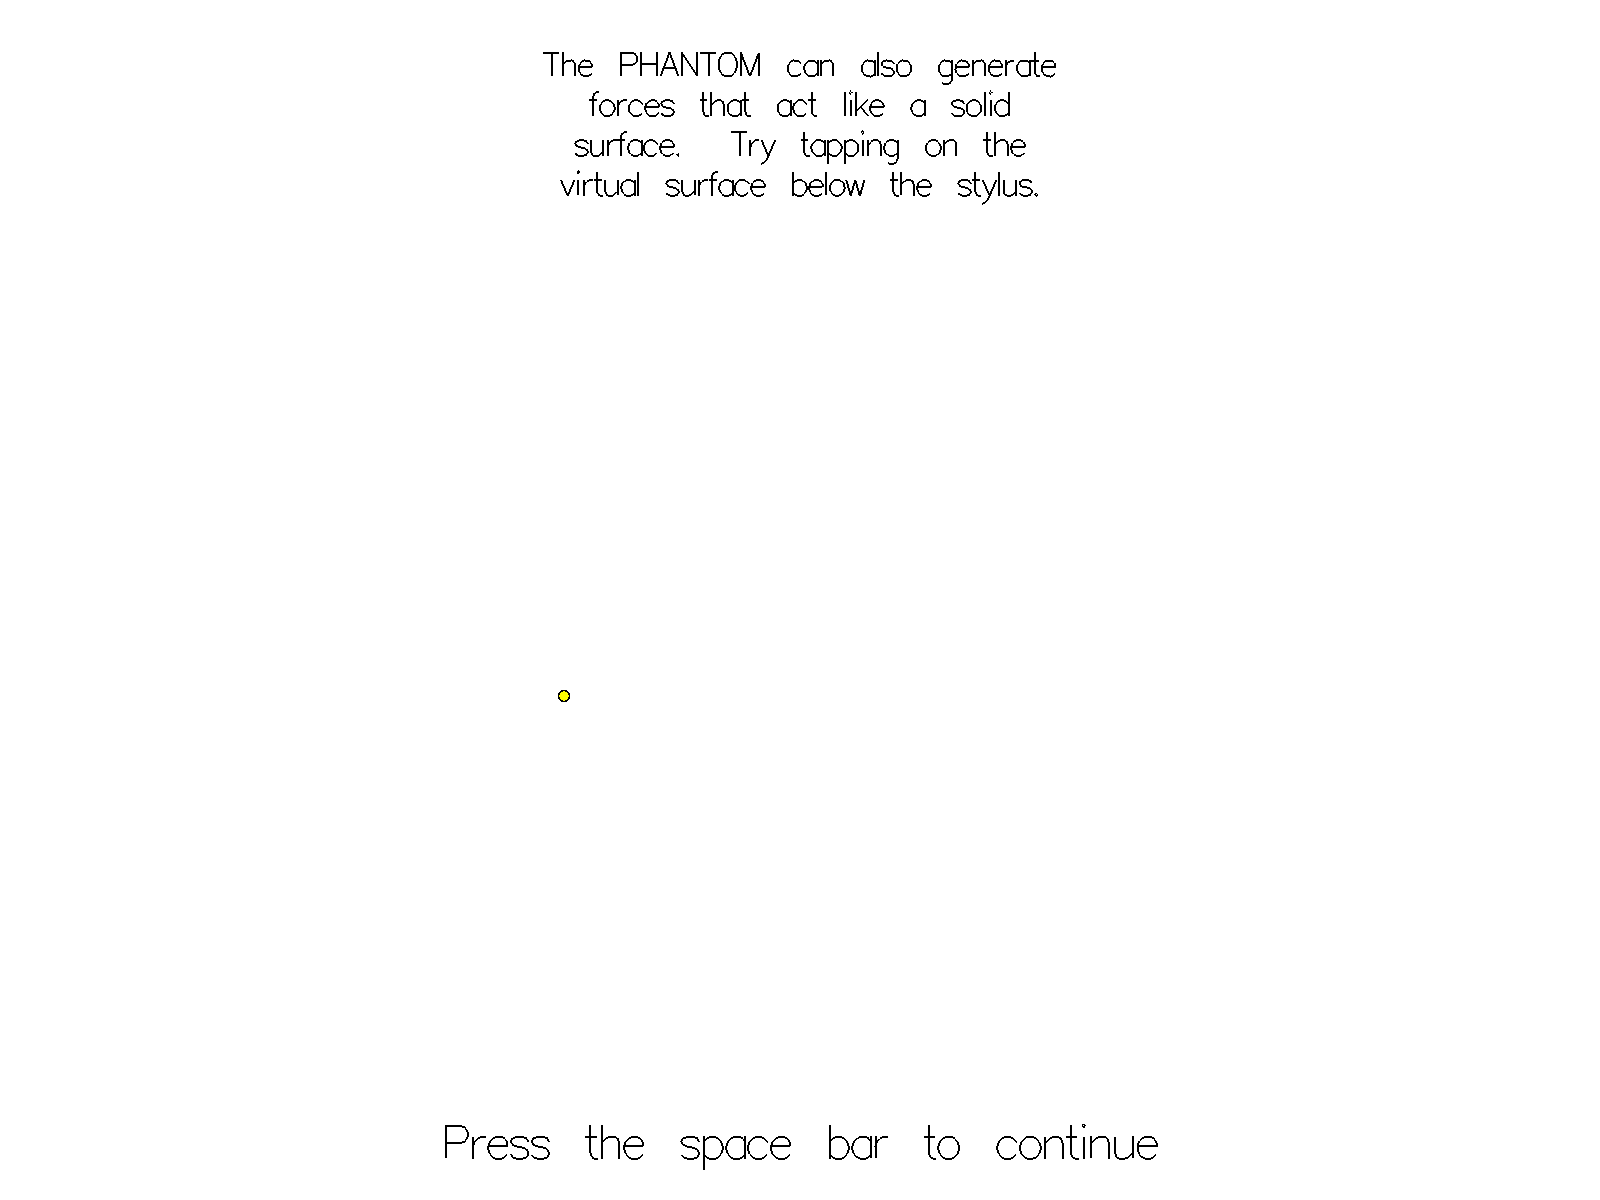
\includegraphics{figures/SolidSurface}}%
}%
\caption[]{}%
\label{fig:instructions3}%
\end{figure}%

\begin{figure}%
\ContinuedFloat%
\centering%
\subfloat[][]{%
\label{subfig:instructionsVirtualWalls}%
\fbox{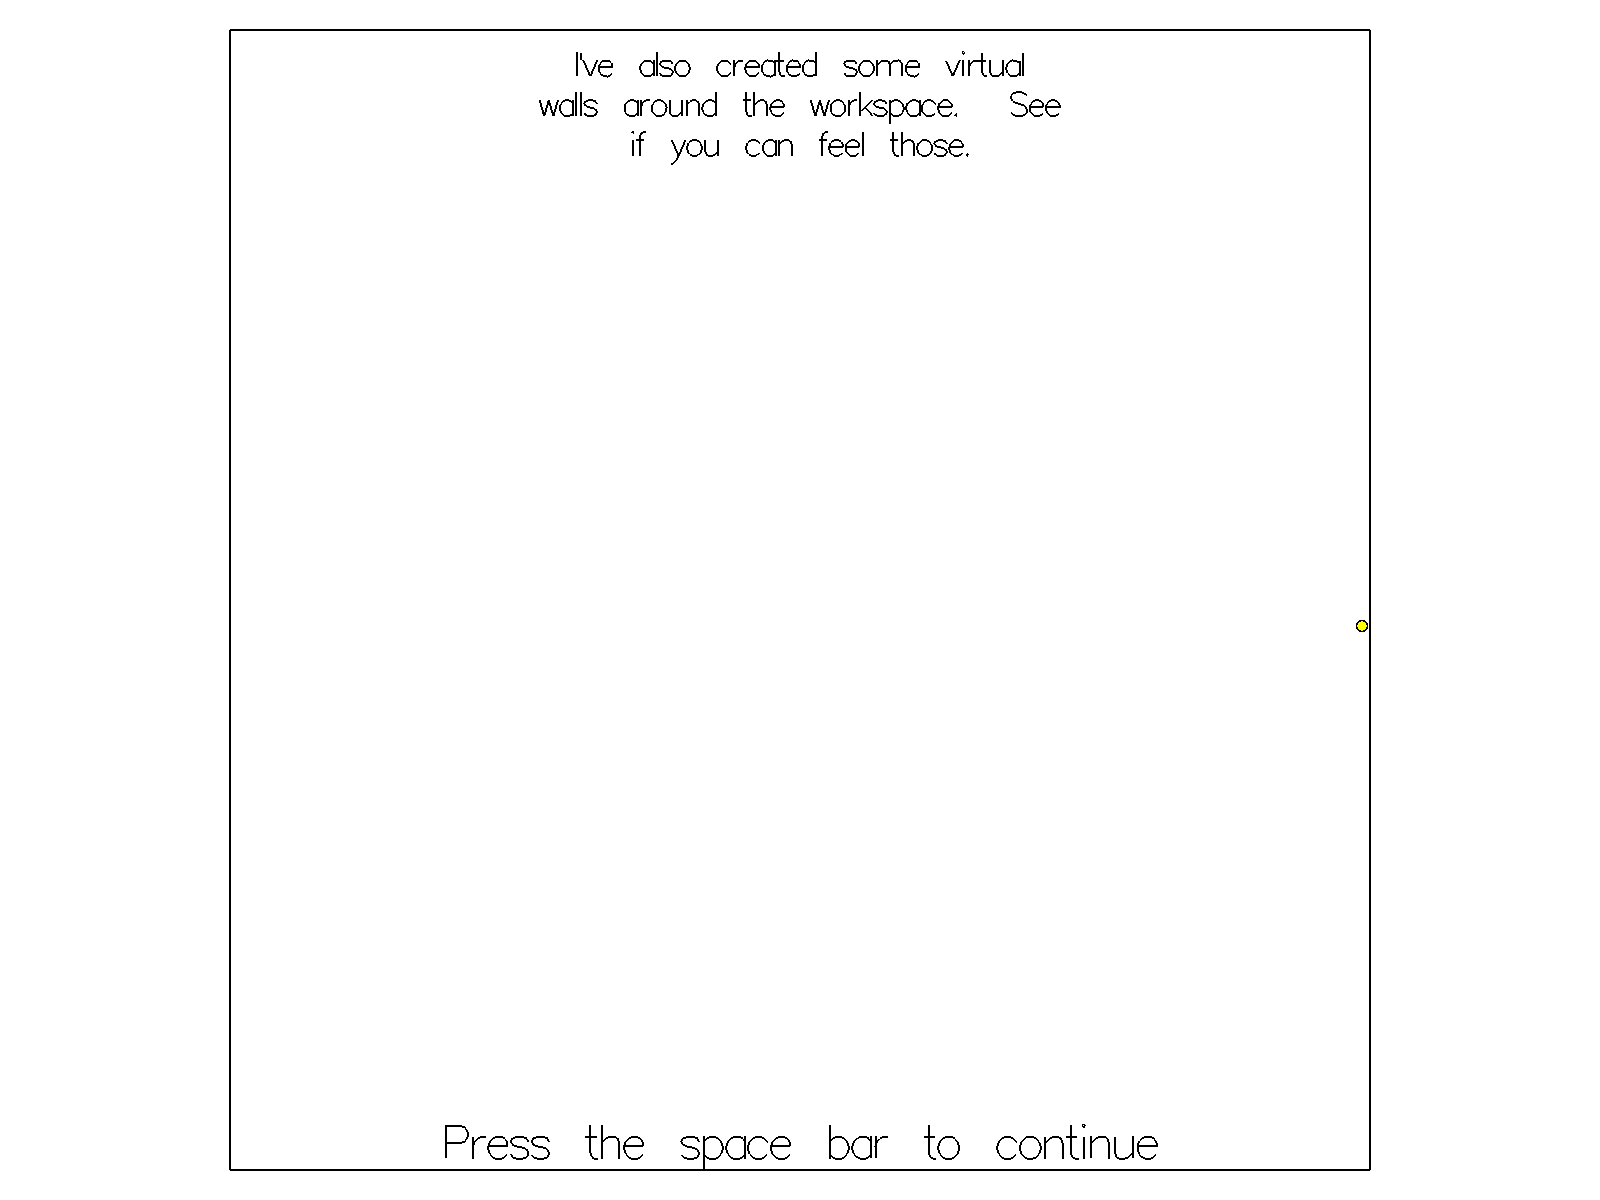
\includegraphics{figures/VirtualWalls}}%
}%
\linebreak%
\subfloat[][]{%
\label{subfig:instructionsTexture}%
\fbox{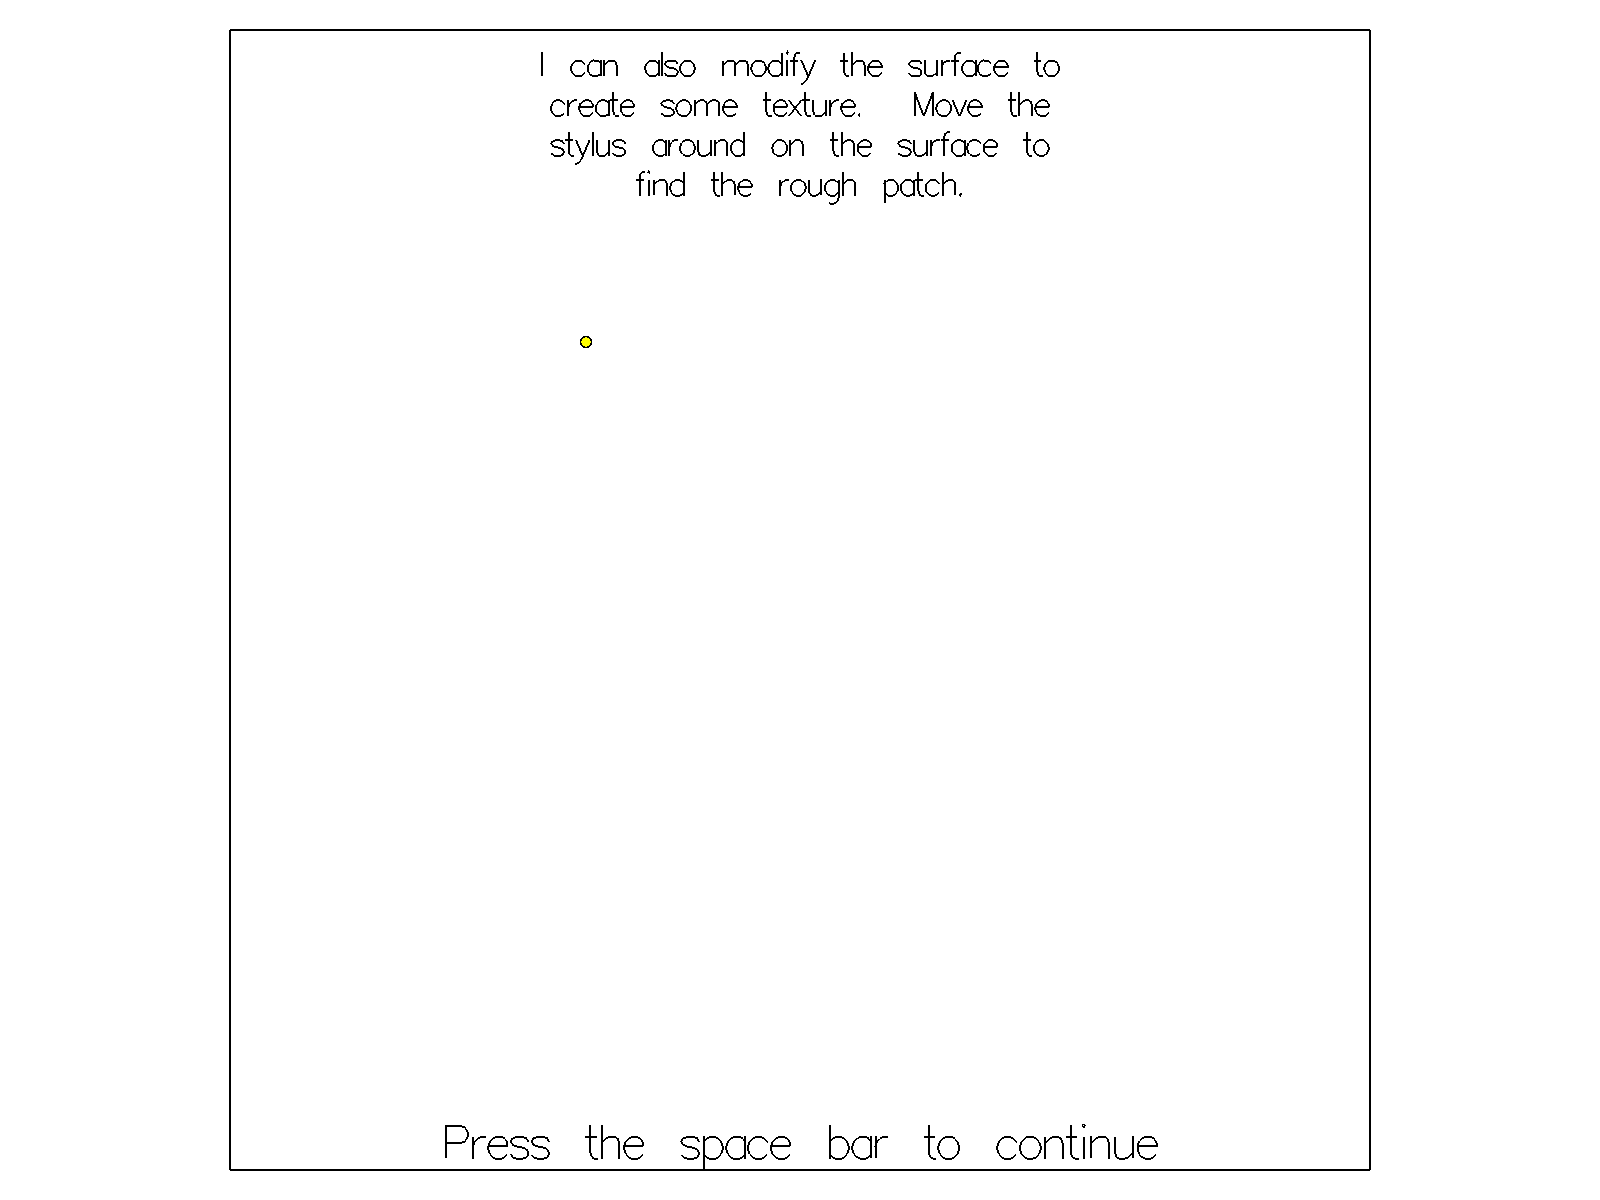
\includegraphics{figures/Texture}}%
}%
\caption[]{}%
\label{fig:instructions4}%
\end{figure}%

\begin{figure}%
\ContinuedFloat%
\centering%
\subfloat[][]{%
\label{subfig:instructionsGroove}%
\fbox{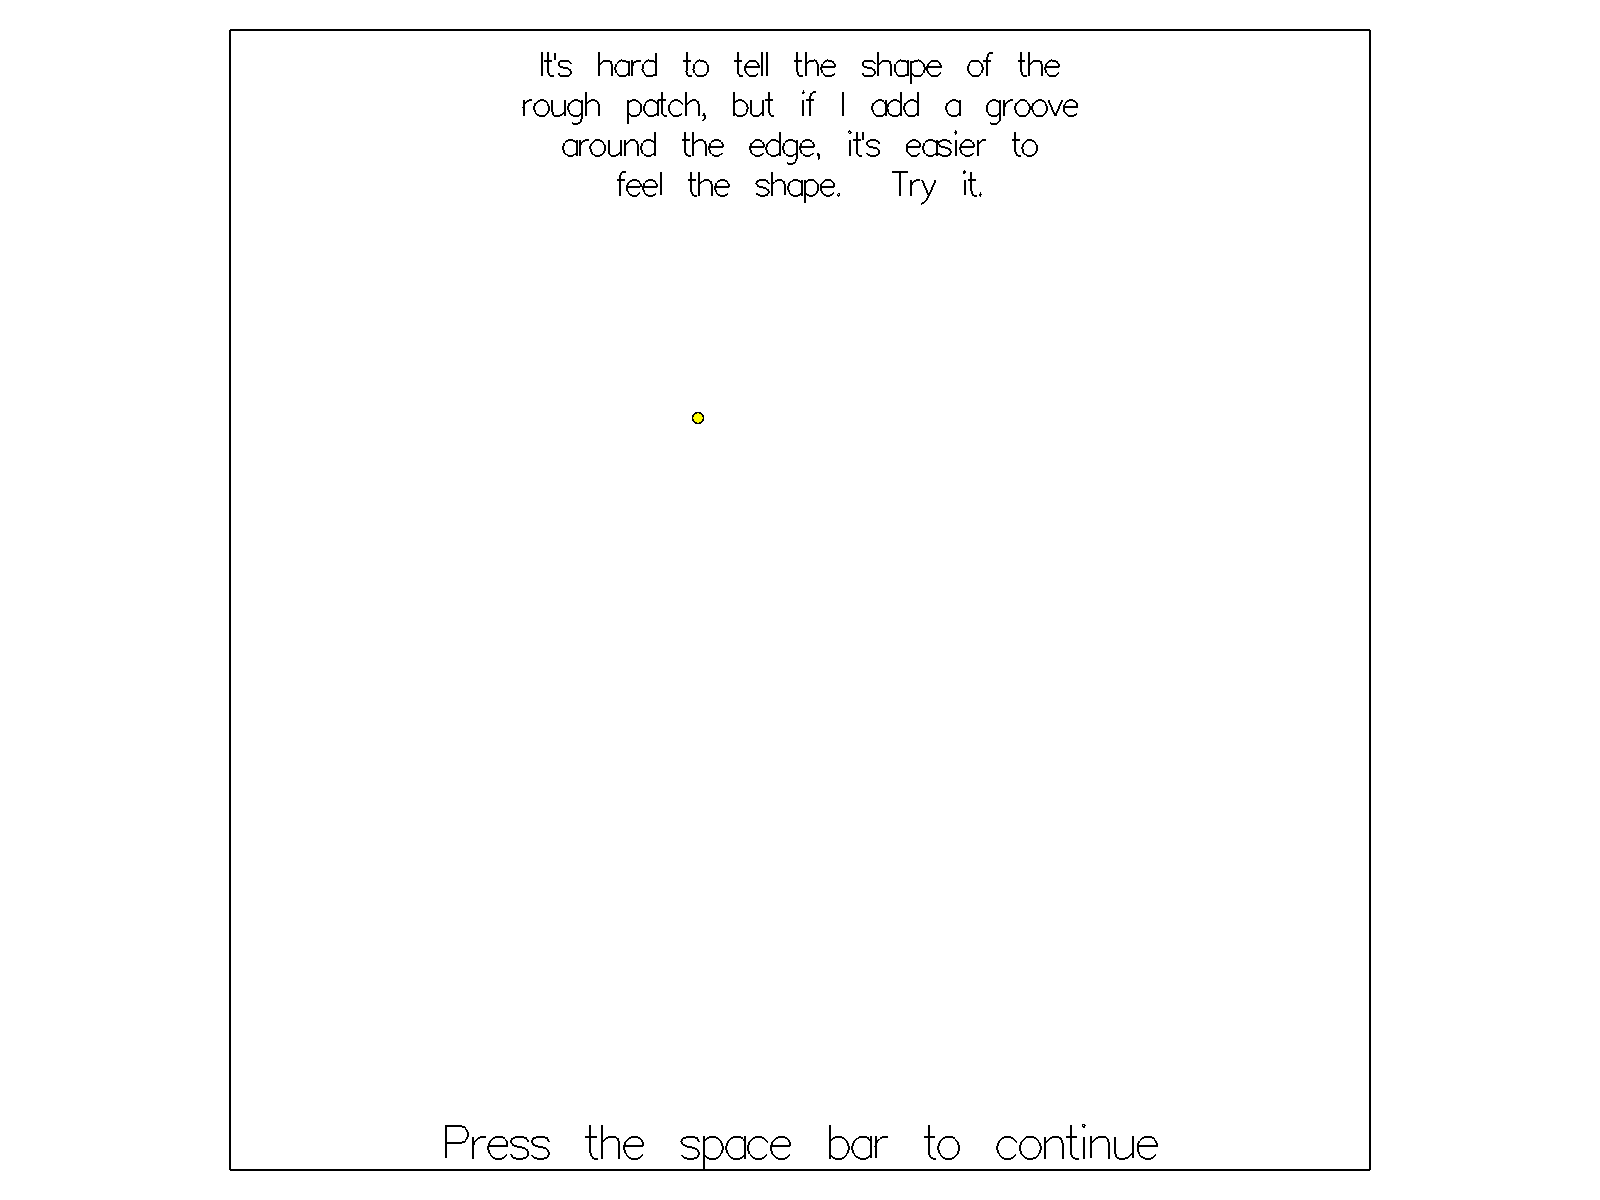
\includegraphics{figures/Groove}}%
}%
\linebreak%
\subfloat[][]{%
\label{subfig:instructionsDent}%
\fbox{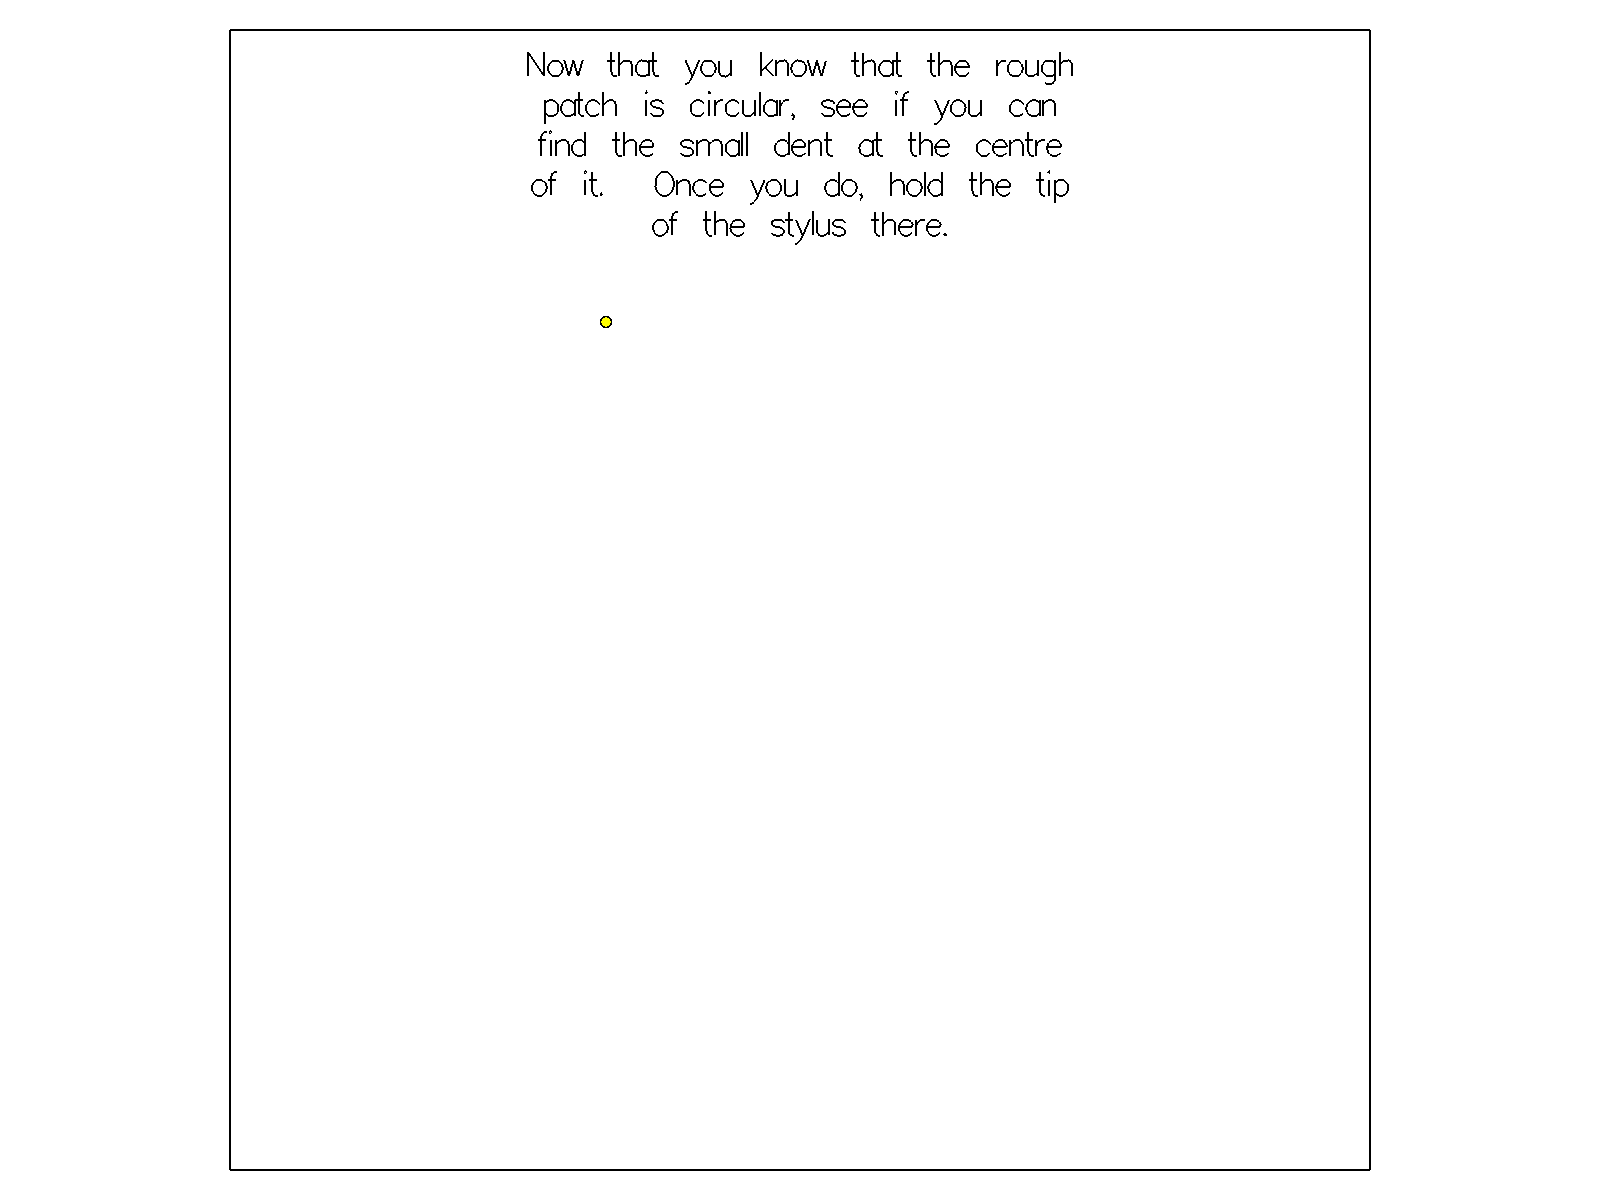
\includegraphics{figures/Dent}}%
}%
\caption[]{}%
\label{fig:instructions5}%
\end{figure}%

\begin{figure}%
\ContinuedFloat%
\centering%
\subfloat[][]{%
\label{subfig:instructionsPatchMoved}%
\fbox{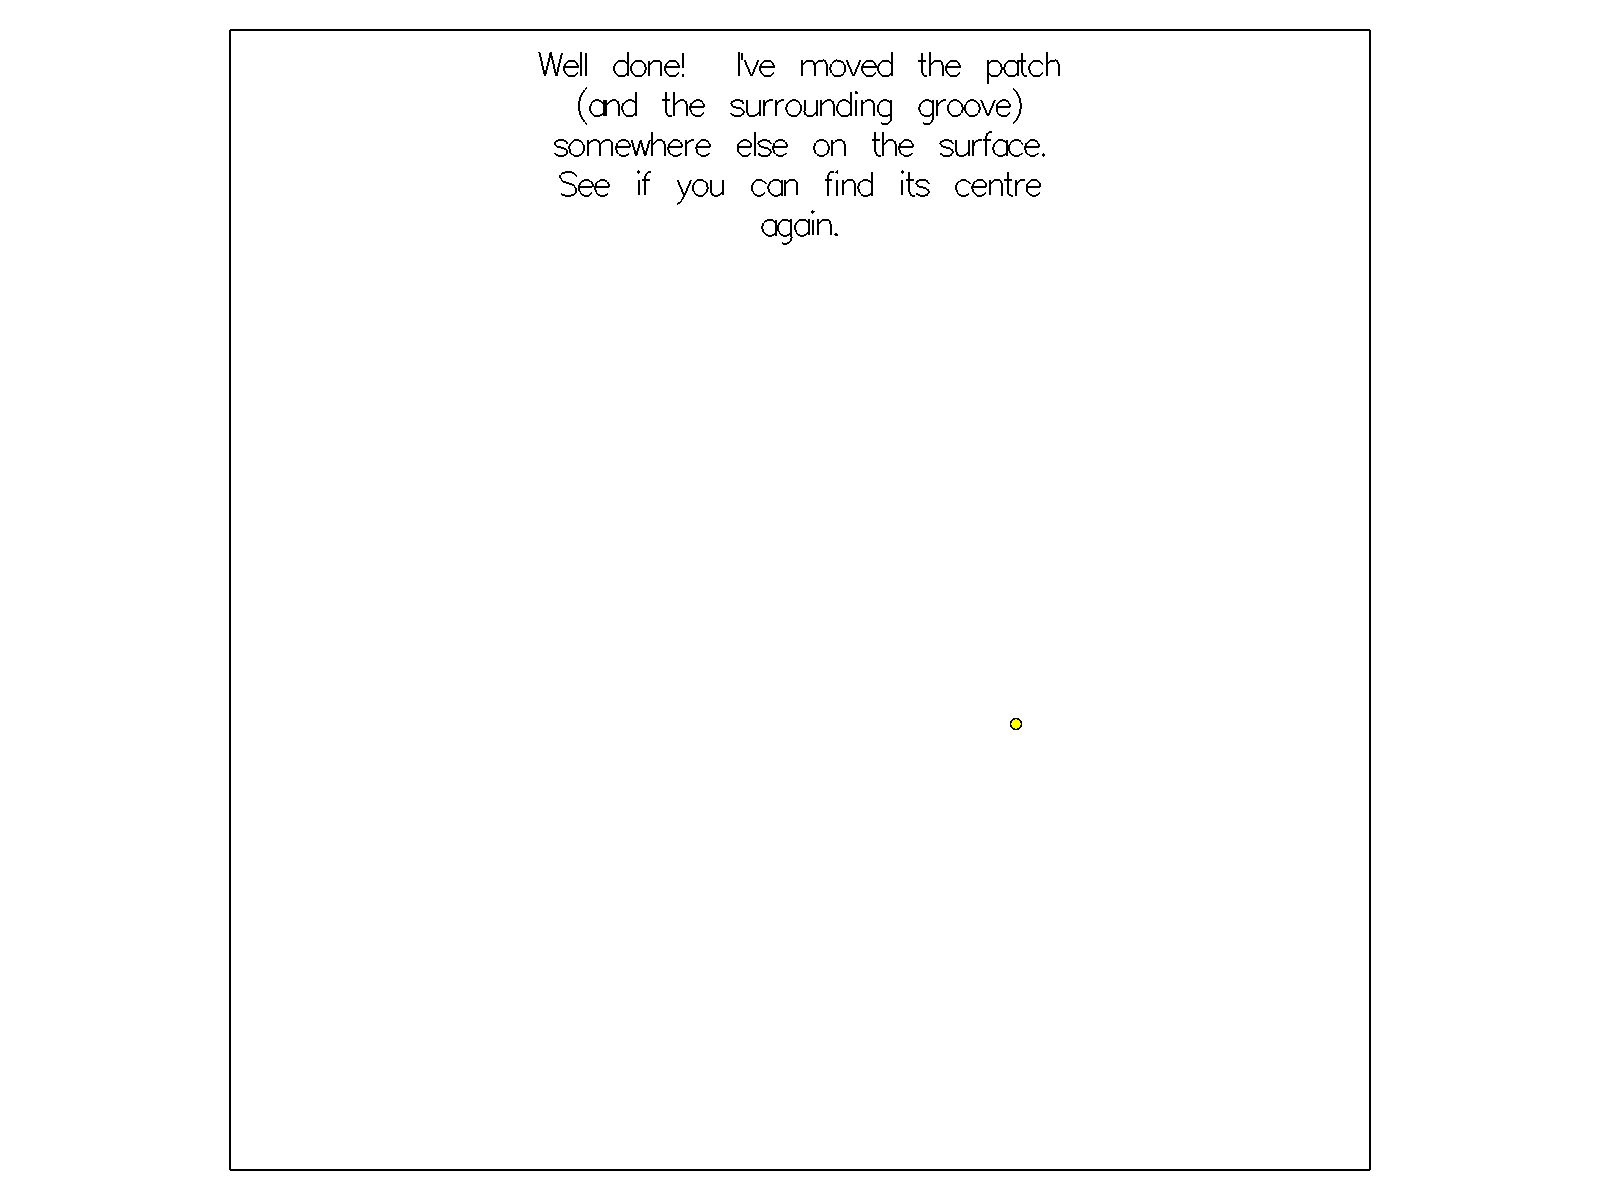
\includegraphics{figures/PatchMoved}}%
}%
\linebreak%
\subfloat[][]{%
\label{subfig:instructionsDifferentTextures}%
\fbox{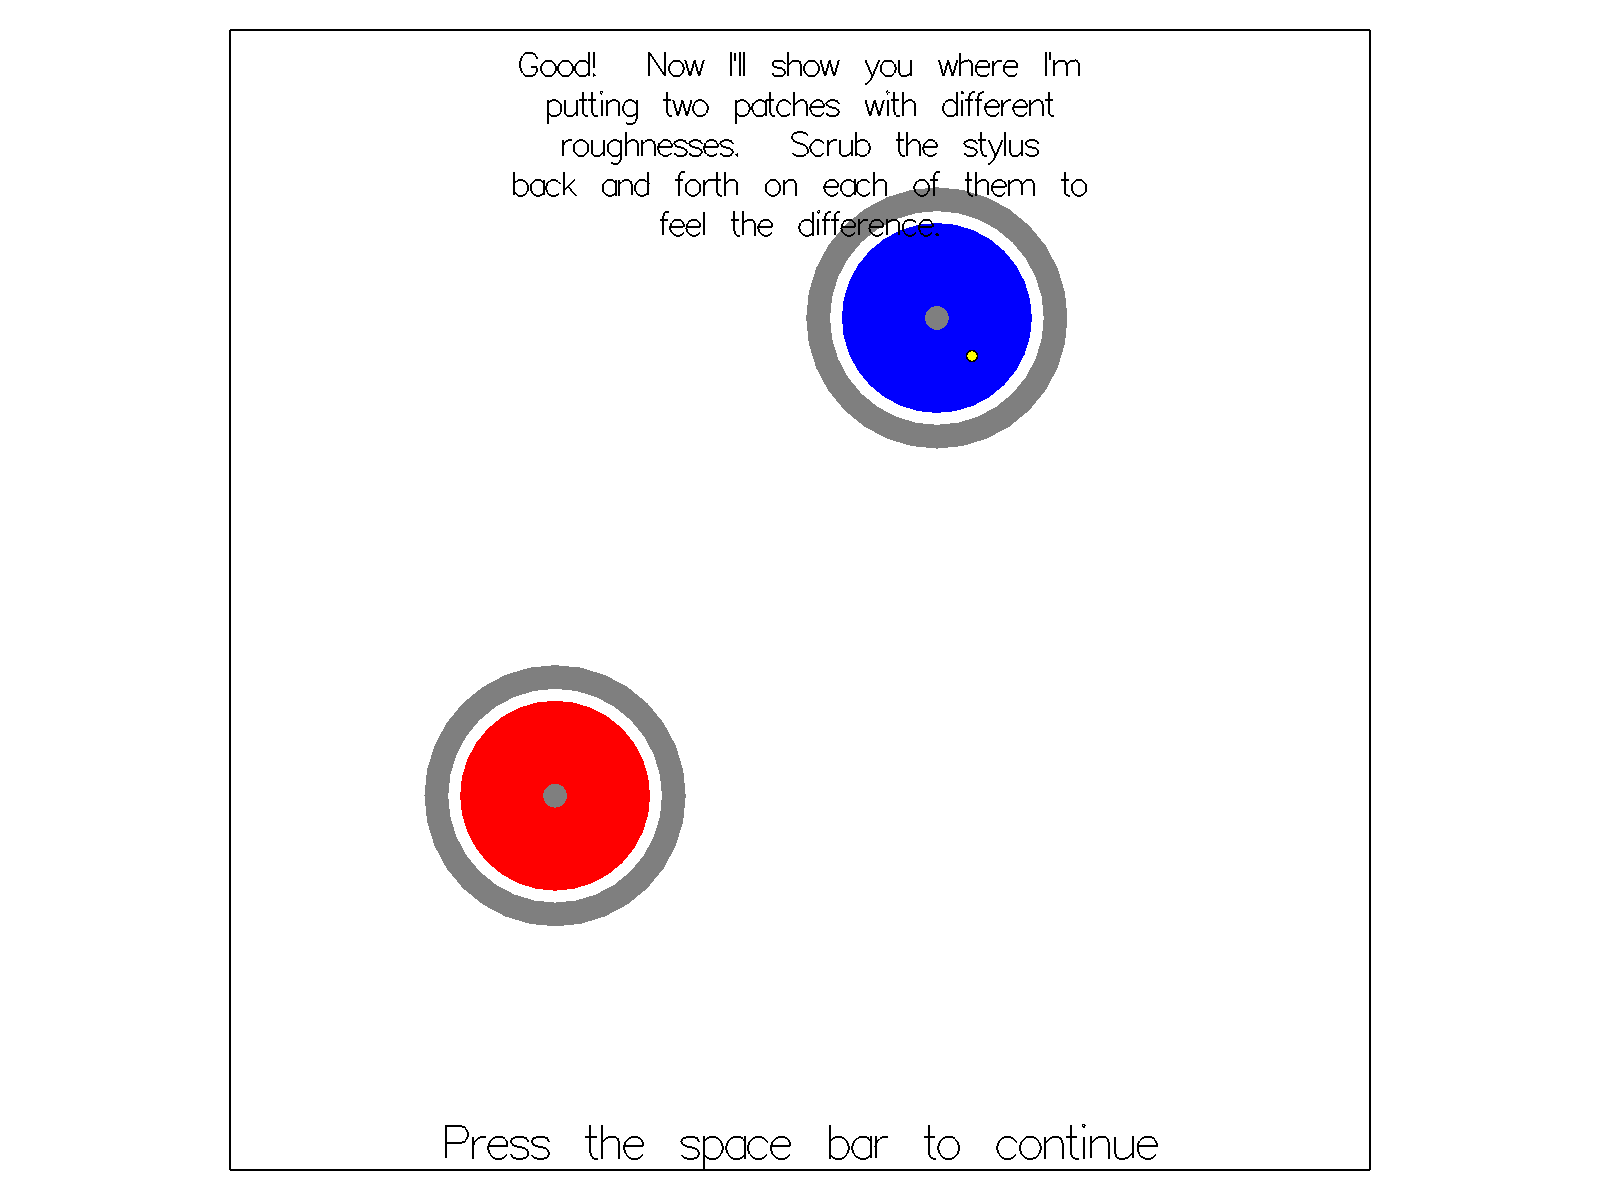
\includegraphics{figures/DifferentTextures}}%
}%
\caption[]{}%
\label{fig:instructions6}%
\end{figure}%

\begin{figure}%
\ContinuedFloat%
\centering%
\subfloat[][]{%
\label{subfig:instructionsBlueIsGood}%
\fbox{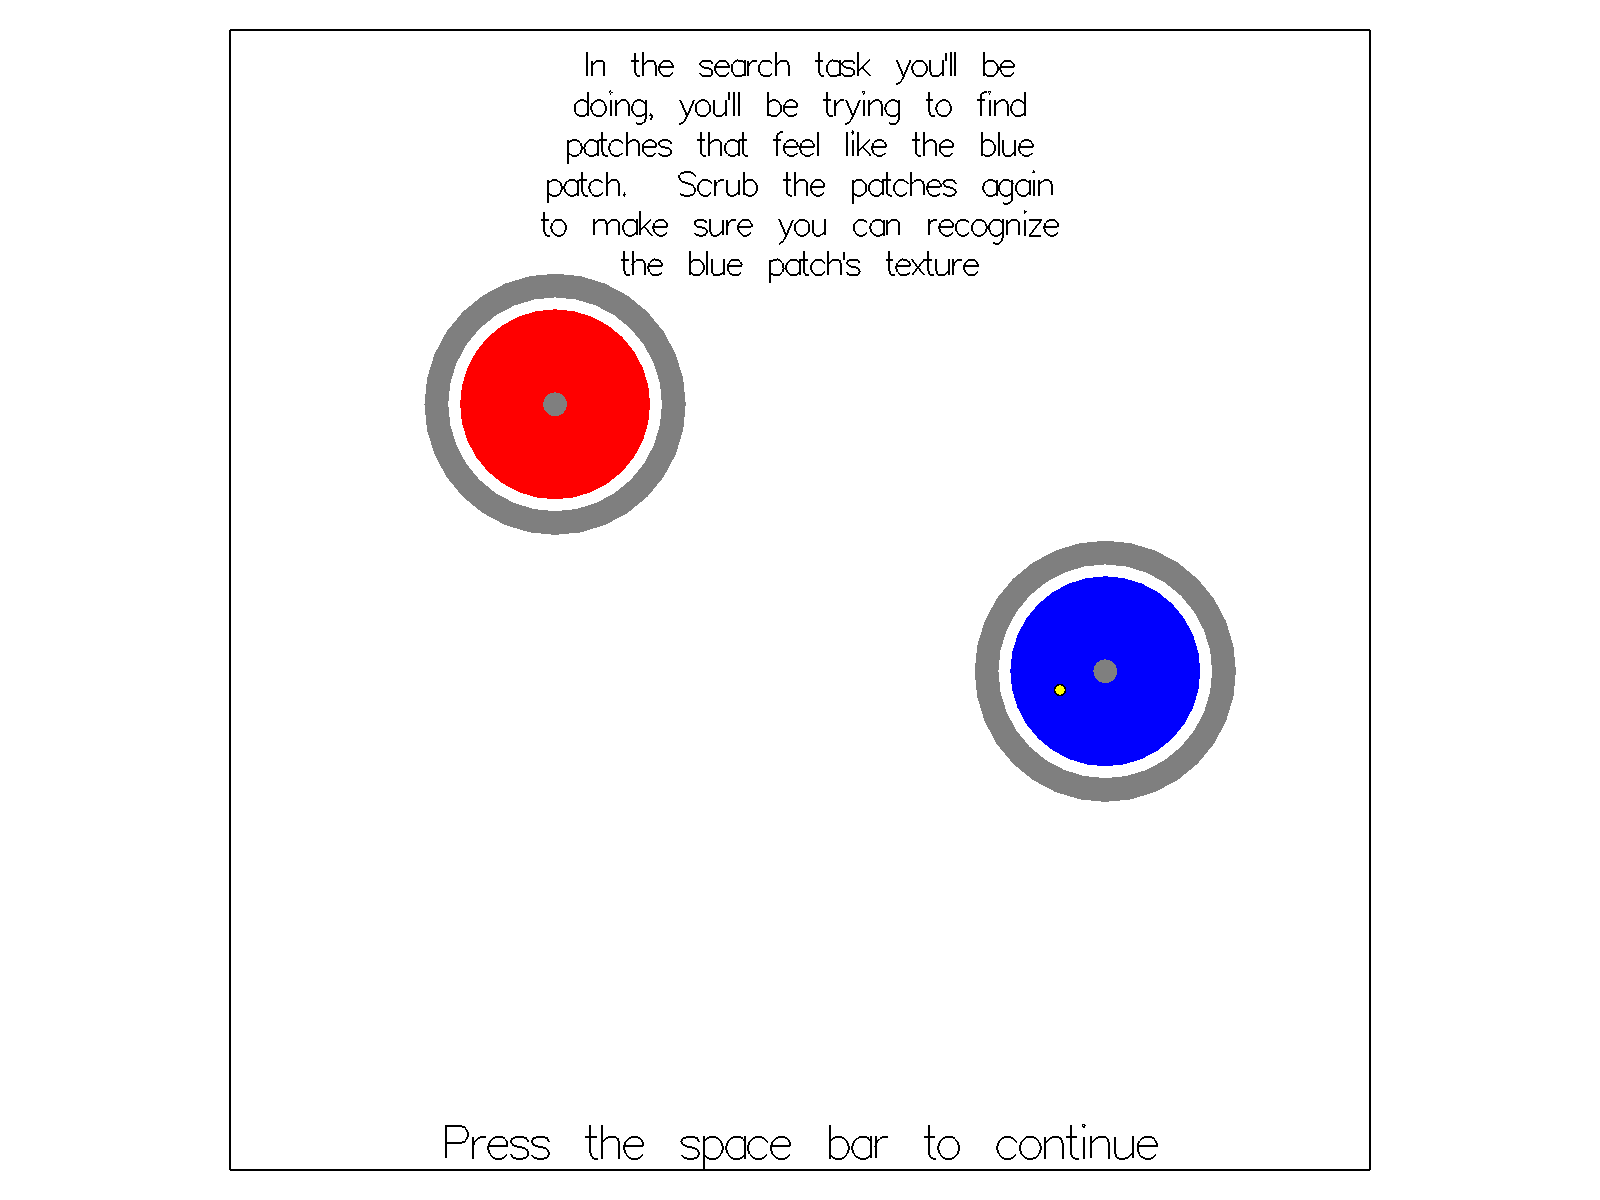
\includegraphics{figures/BlueIsGood}}%
}%
\linebreak%
\subfloat[][]{%
\label{subfig:instructionsTaskExplanation}%
\fbox{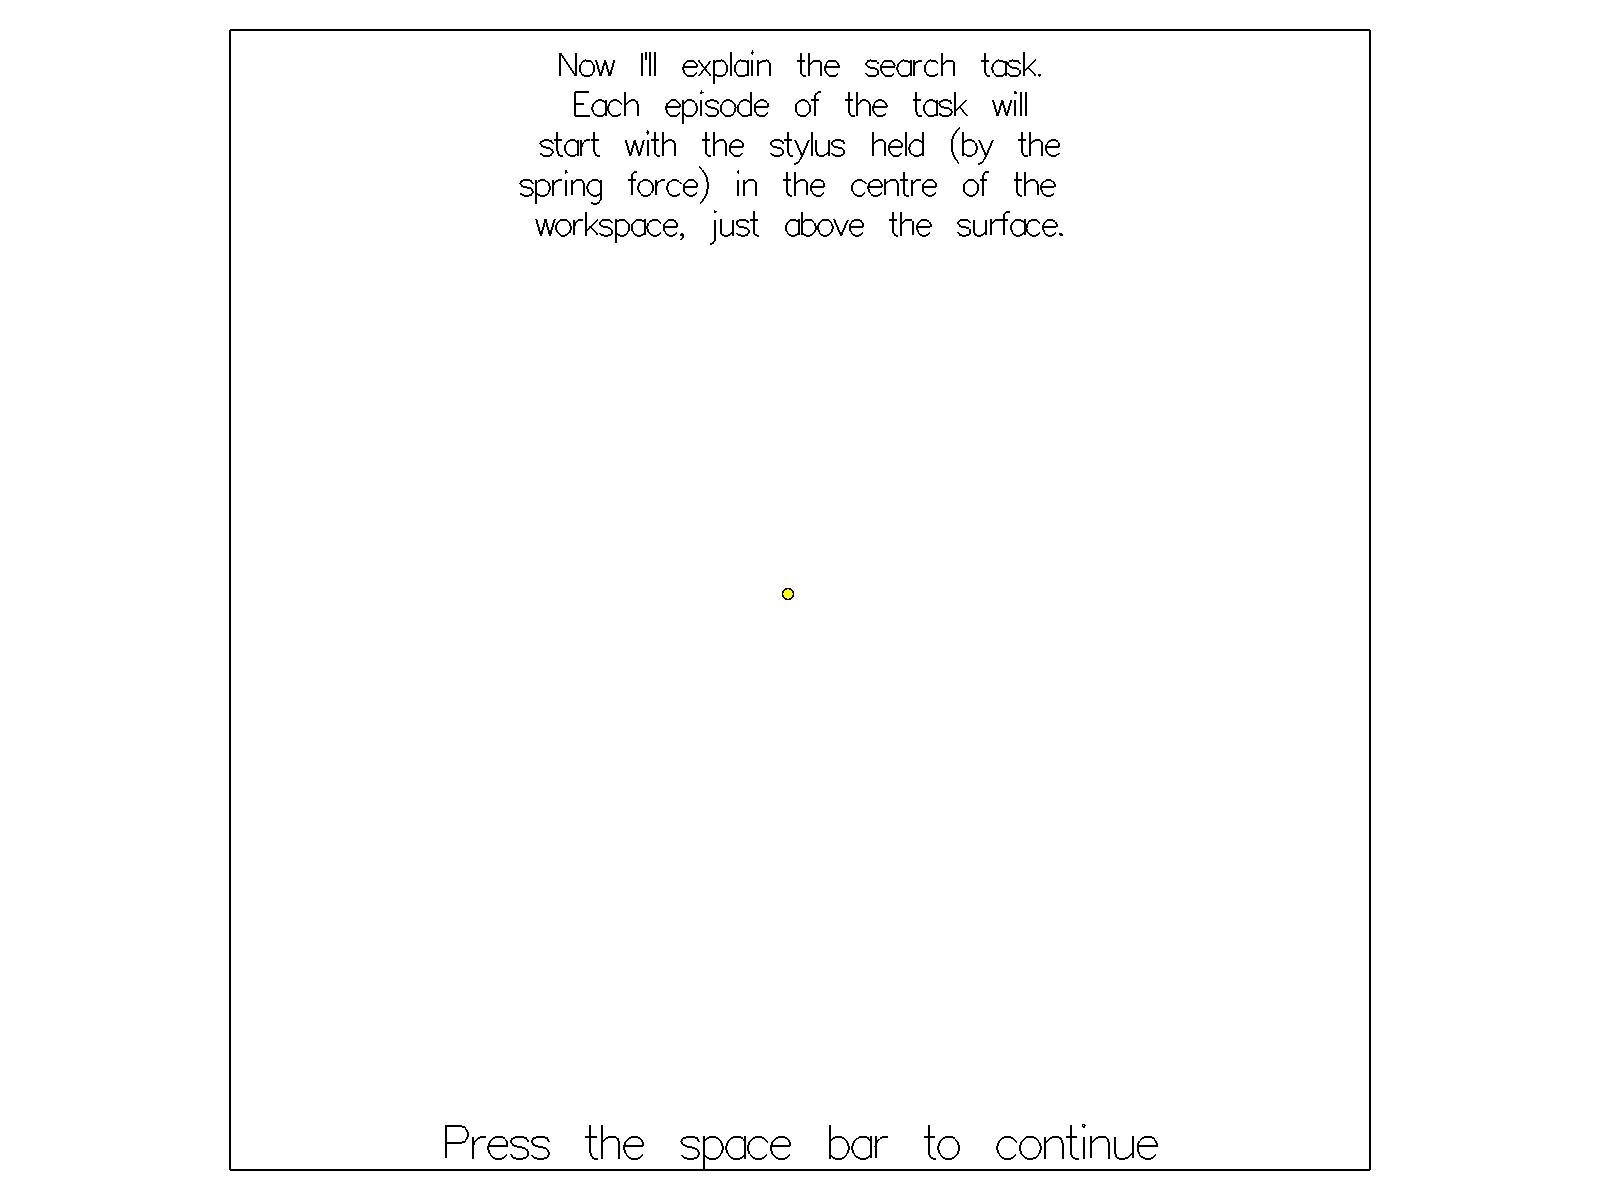
\includegraphics{figures/TaskExplanation}}%
}%
\caption[]{}%
\label{fig:instructions7}%
\end{figure}%

\begin{figure}%
\ContinuedFloat%
\centering%
\subfloat[][]{%
\label{subfig:instructionsEpisodeBegins}%
\fbox{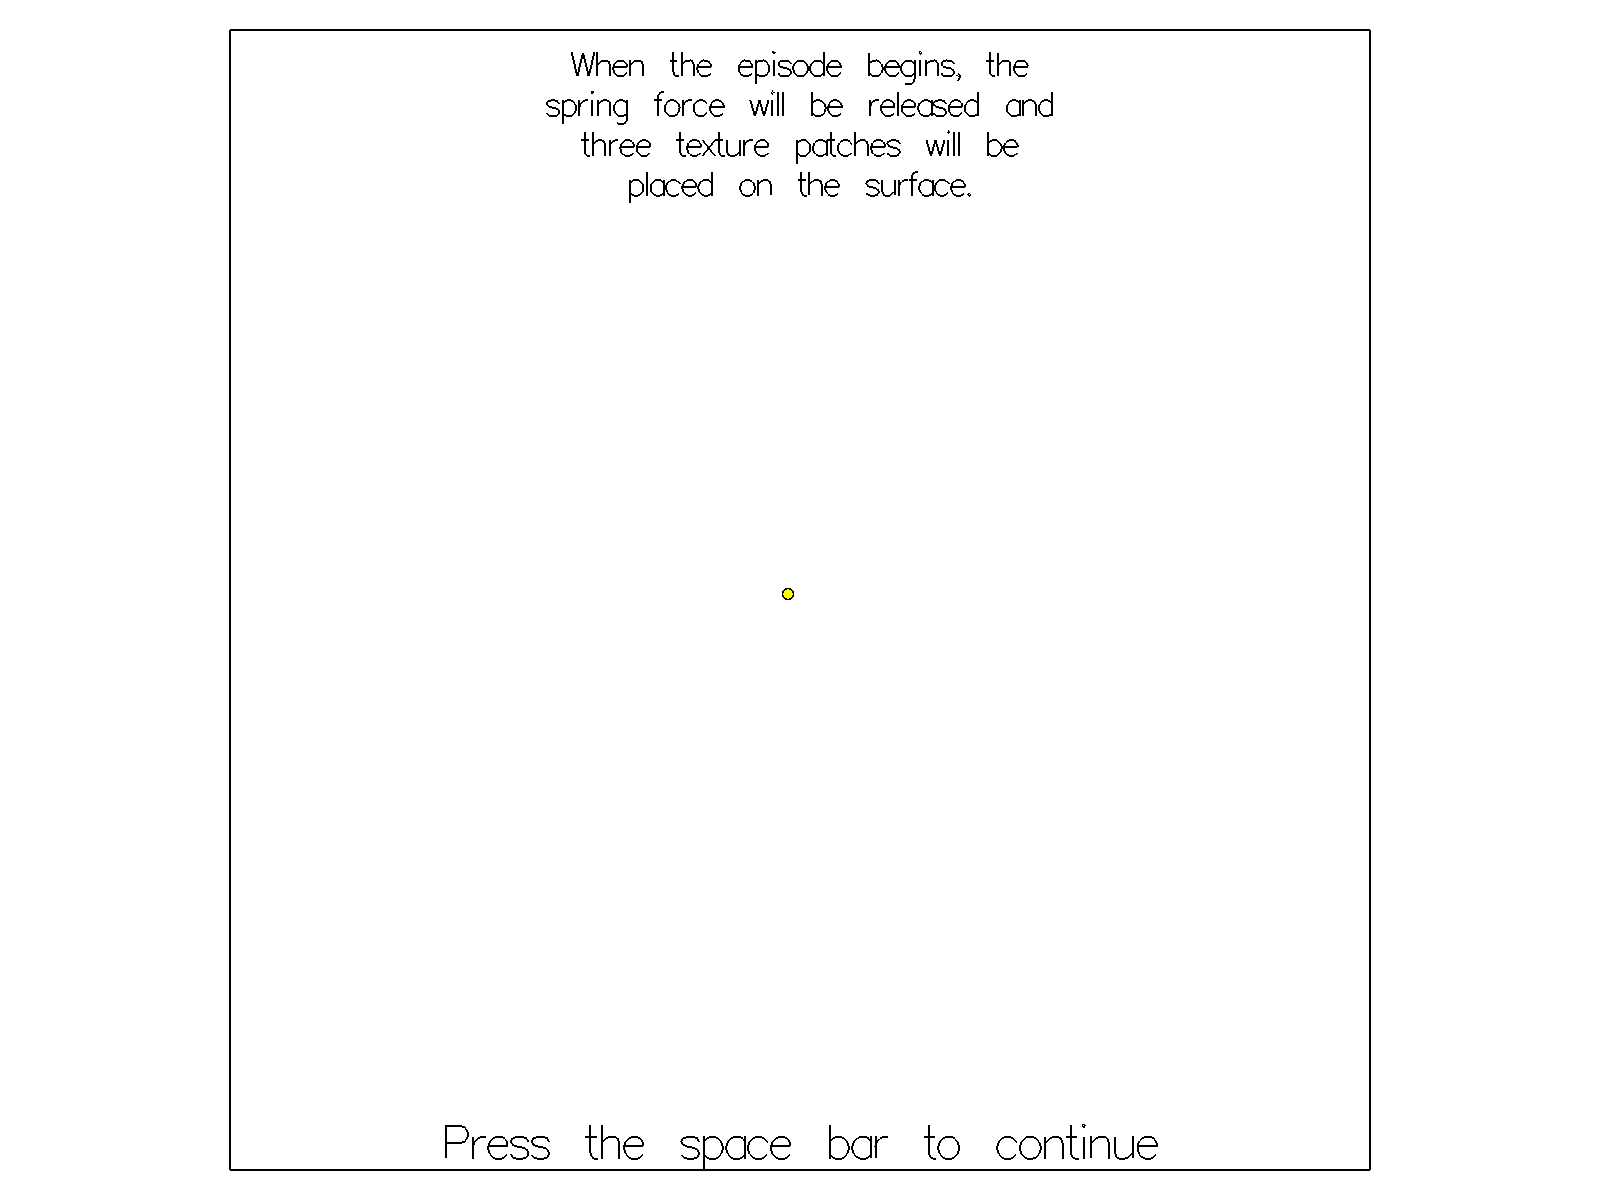
\includegraphics{figures/EpisodeBegins}}%
}%
\linebreak%
\subfloat[][]{%
\label{subfig:instructionsStimulusComposition}%
\fbox{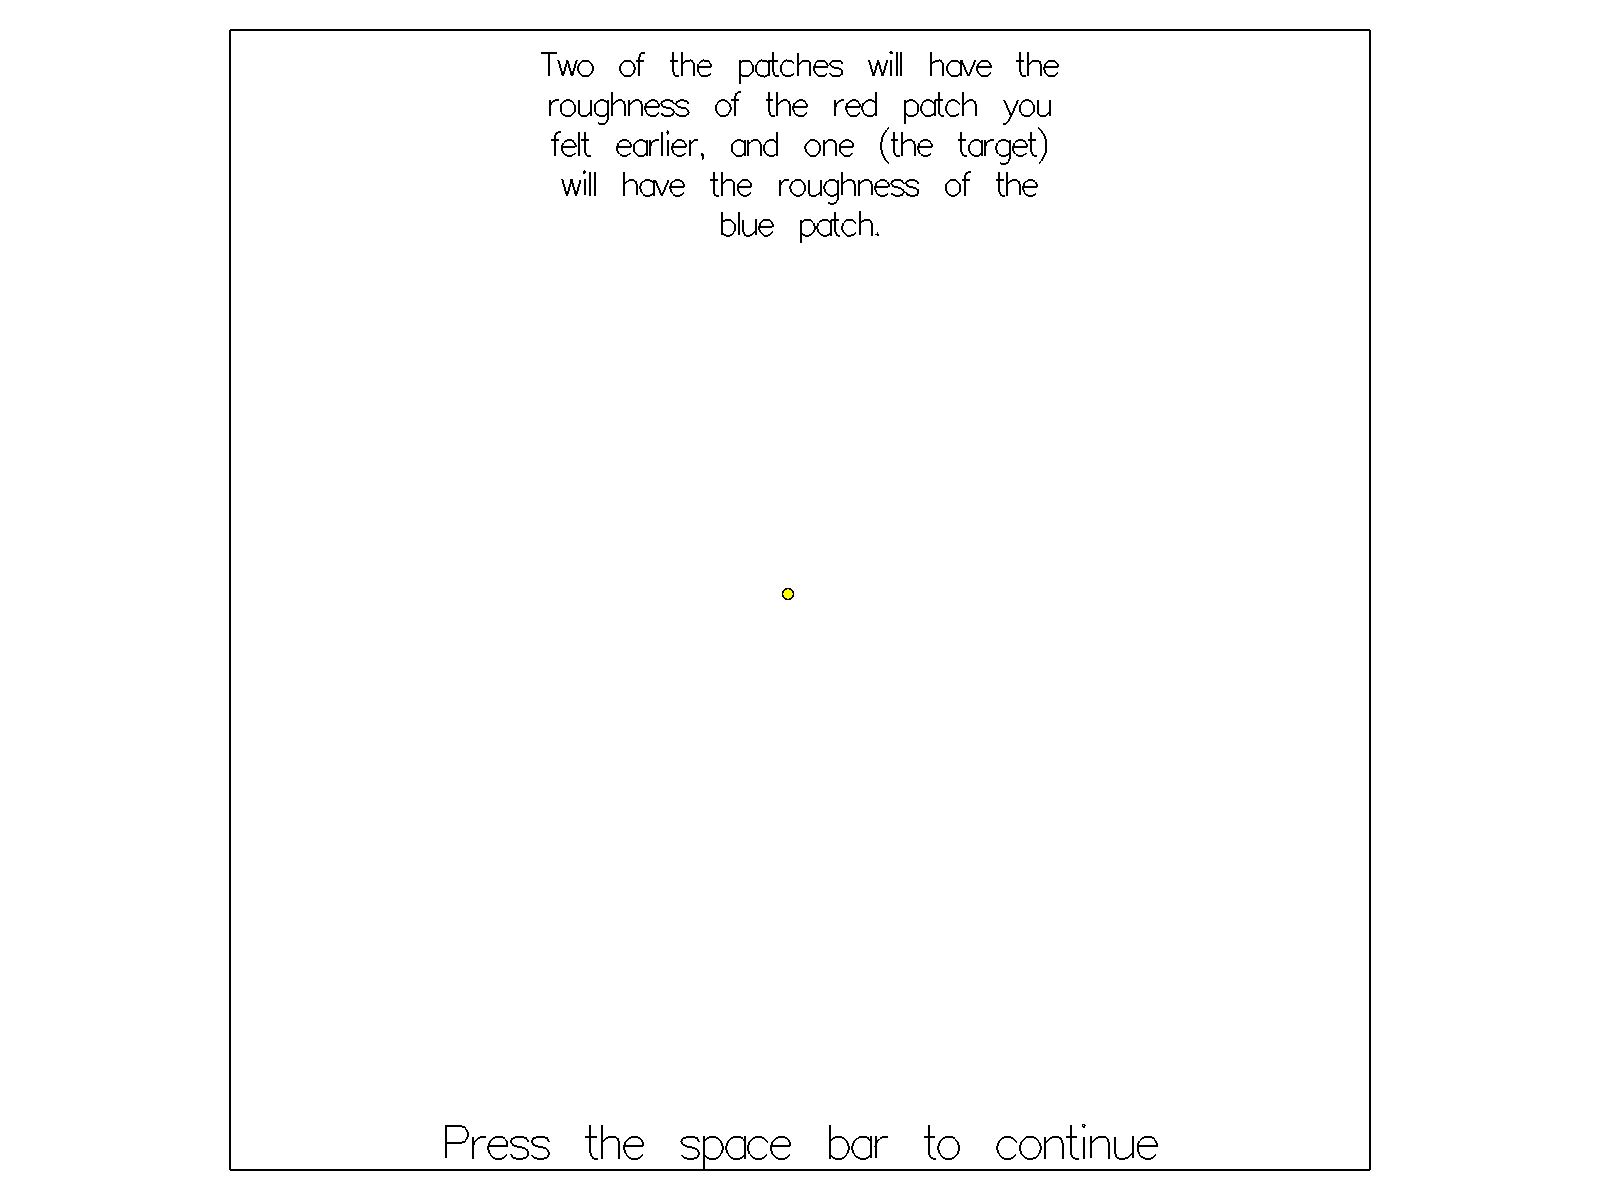
\includegraphics{figures/StimulusComposition}}%
}%
\caption[]{}%
\label{fig:instructions8}%
\end{figure}%

\begin{figure}%
\ContinuedFloat%
\centering%
\subfloat[][]{%
\label{subfig:instructionsStimulusArrangement}%
\fbox{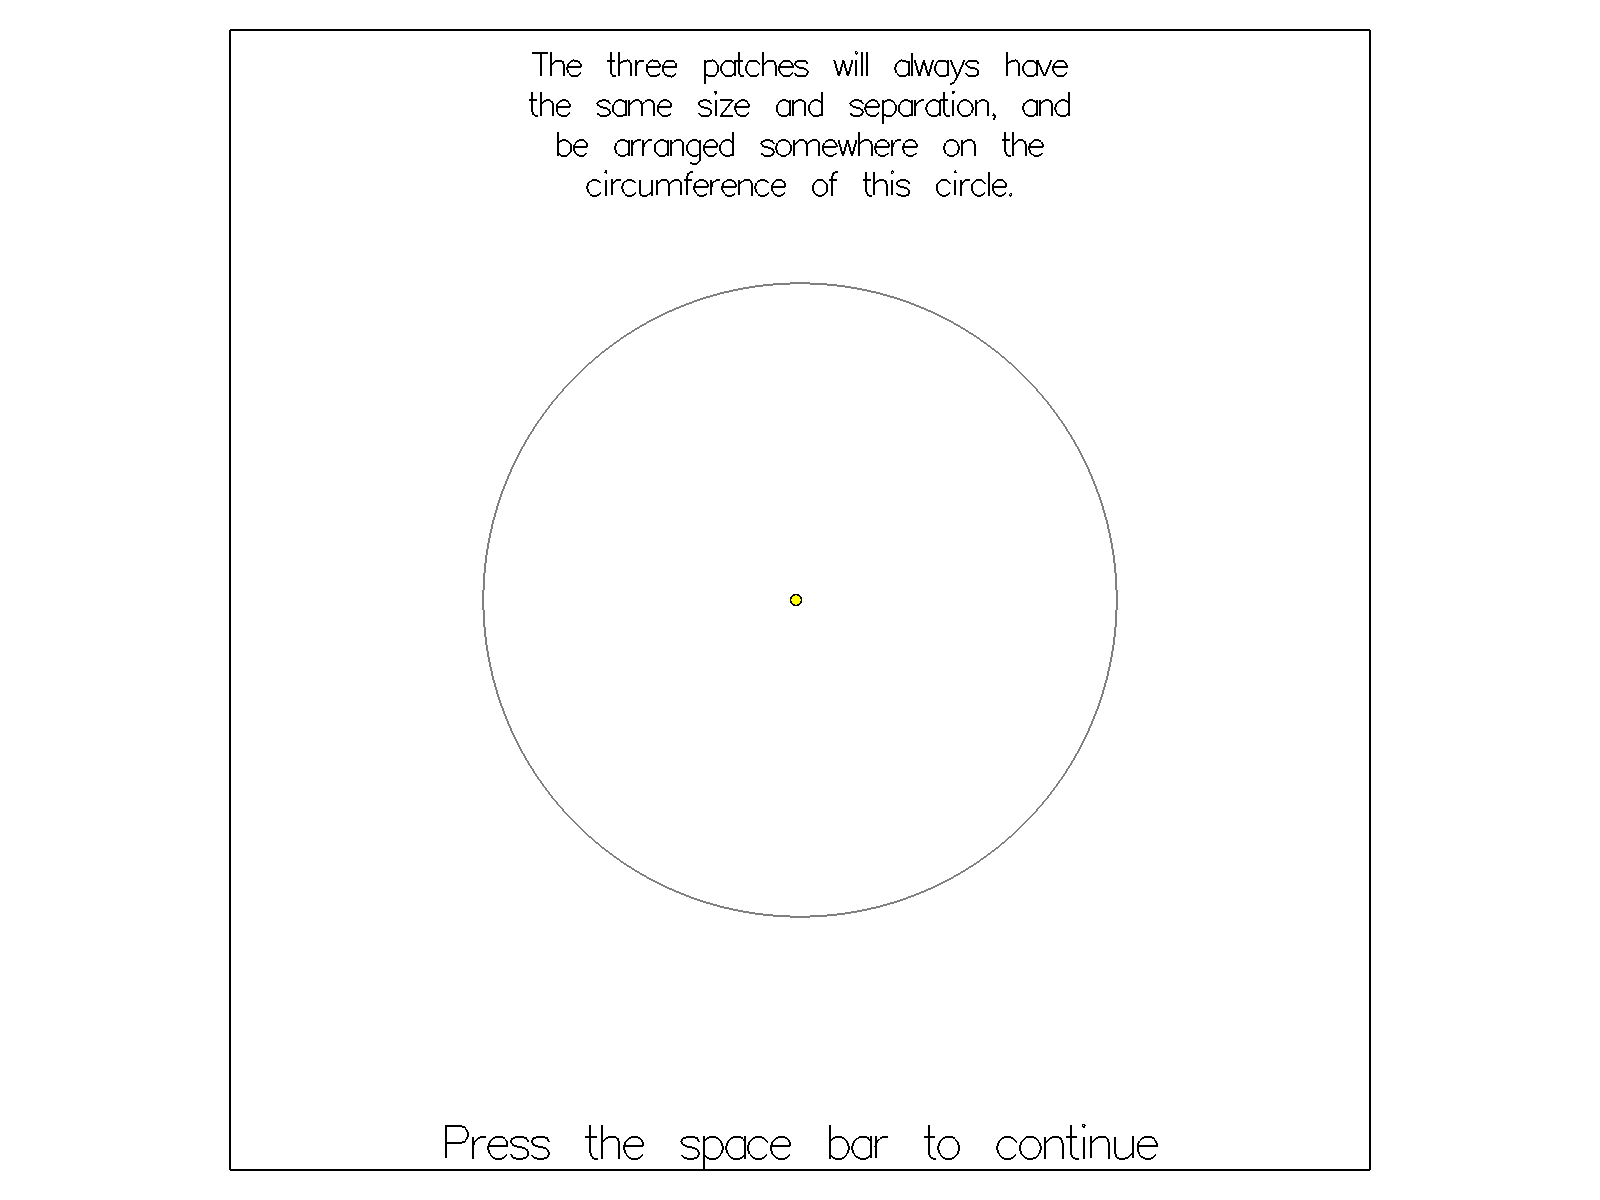
\includegraphics{figures/StimulusArrangement}}%
}%
\linebreak%
\subfloat[][]{%
\label{subfig:instructionsSearchProcedure}%
\fbox{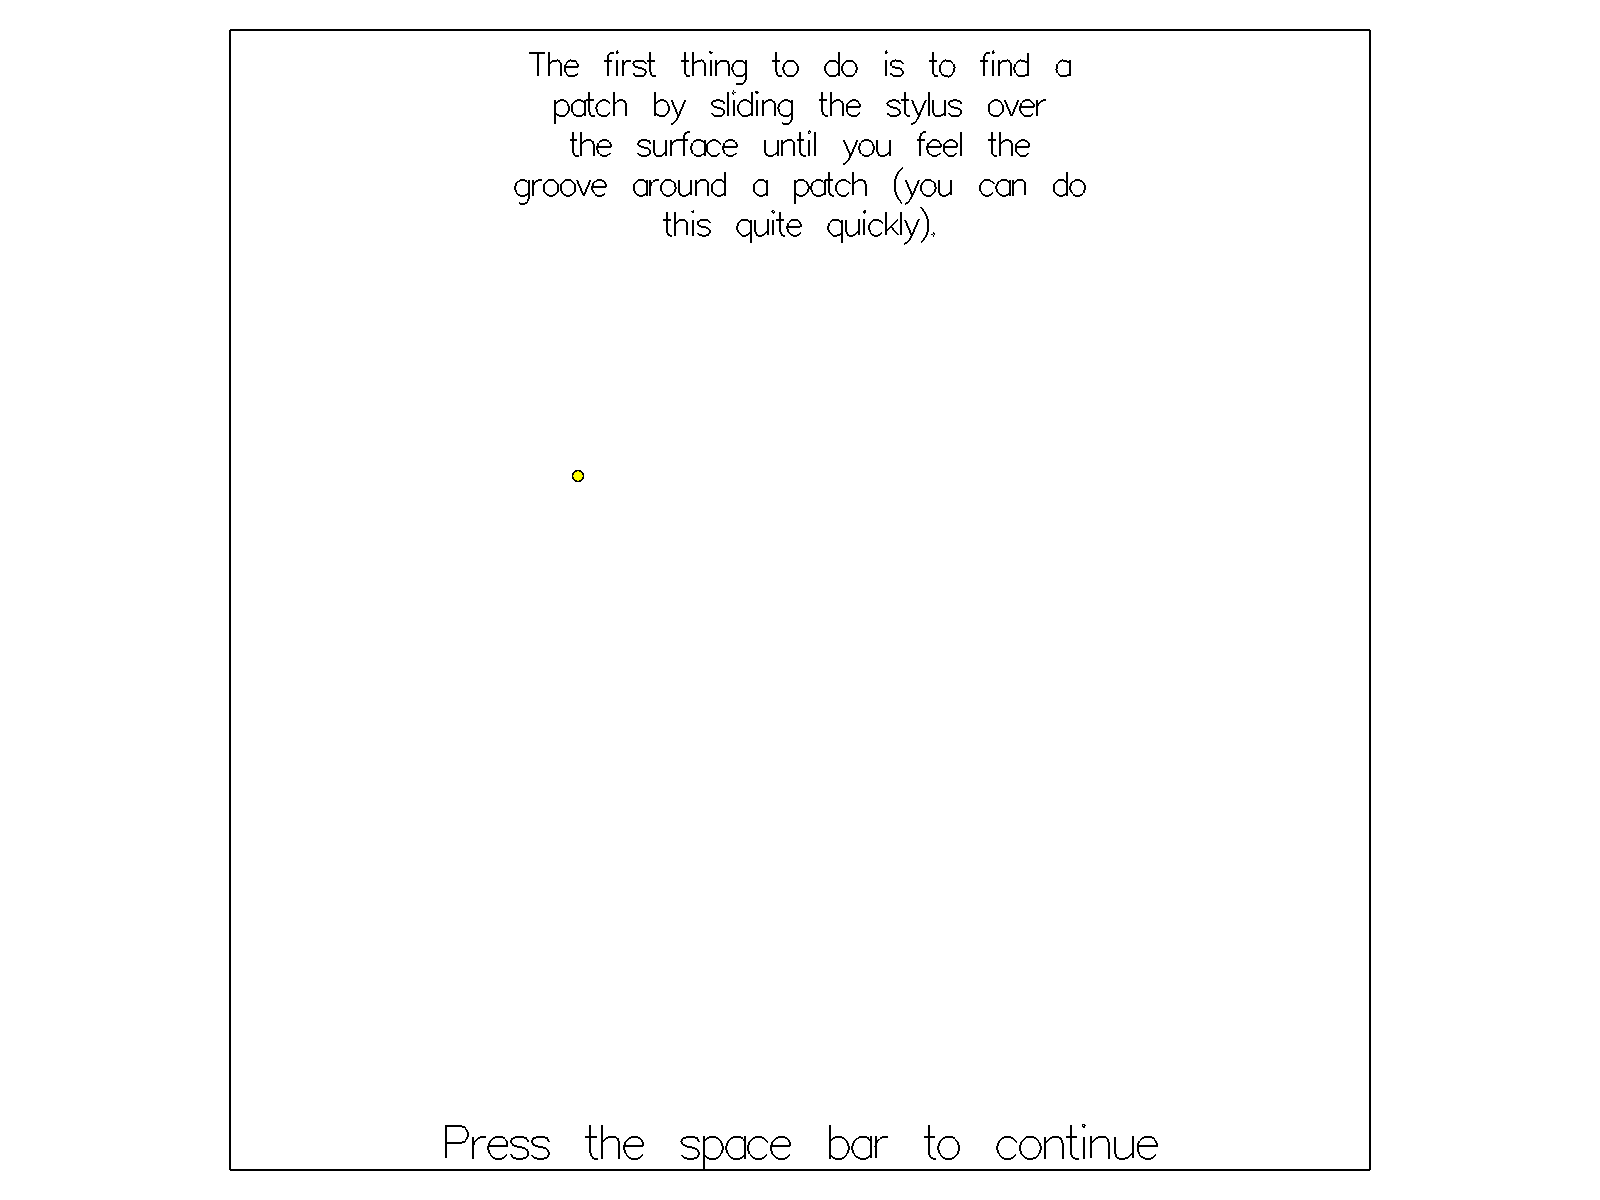
\includegraphics{figures/SearchProcedure}}%
}%
\caption[]{}%
\label{fig:instructions9}%
\end{figure}%

\begin{figure}%
\ContinuedFloat%
\centering%
\subfloat[][]{%
\label{subfig:instructionsIdentificationProcedure}%
\fbox{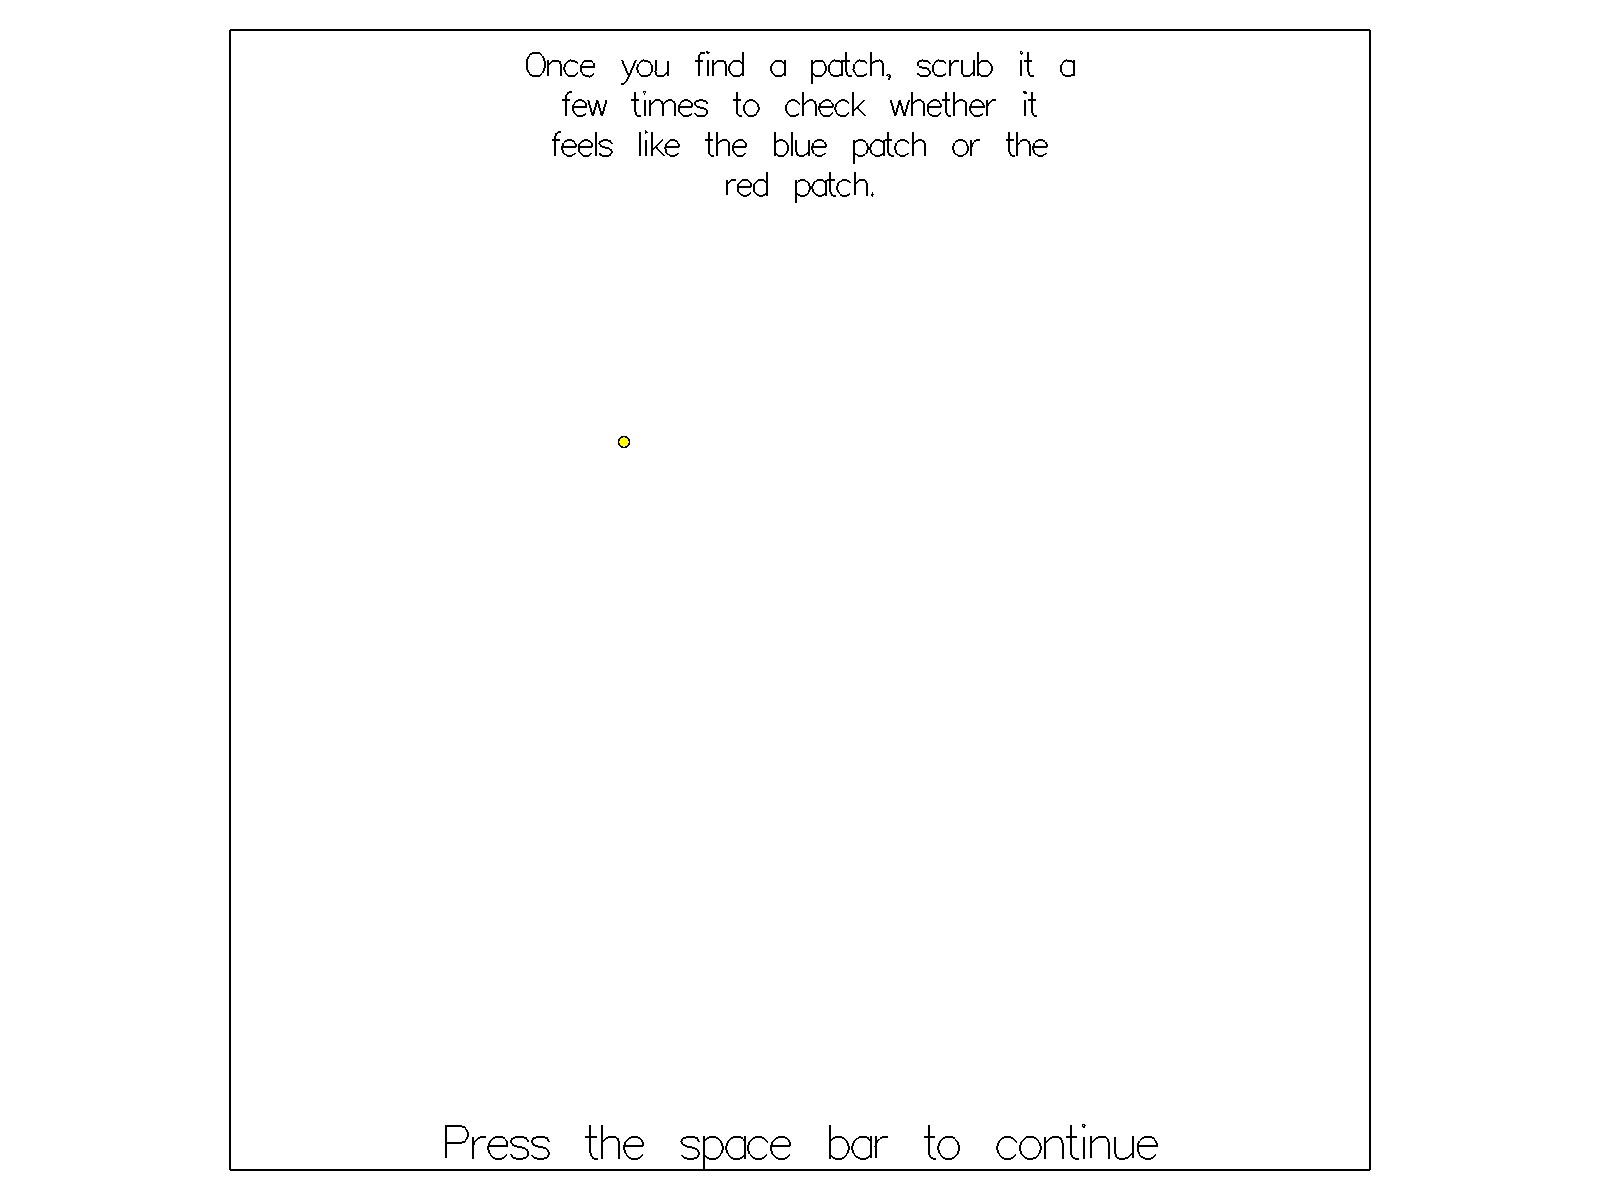
\includegraphics{figures/IdentificationProcedure}}%
}%
\linebreak%
\subfloat[][]{%
\label{subfig:instructionsDecisionRed}%
\fbox{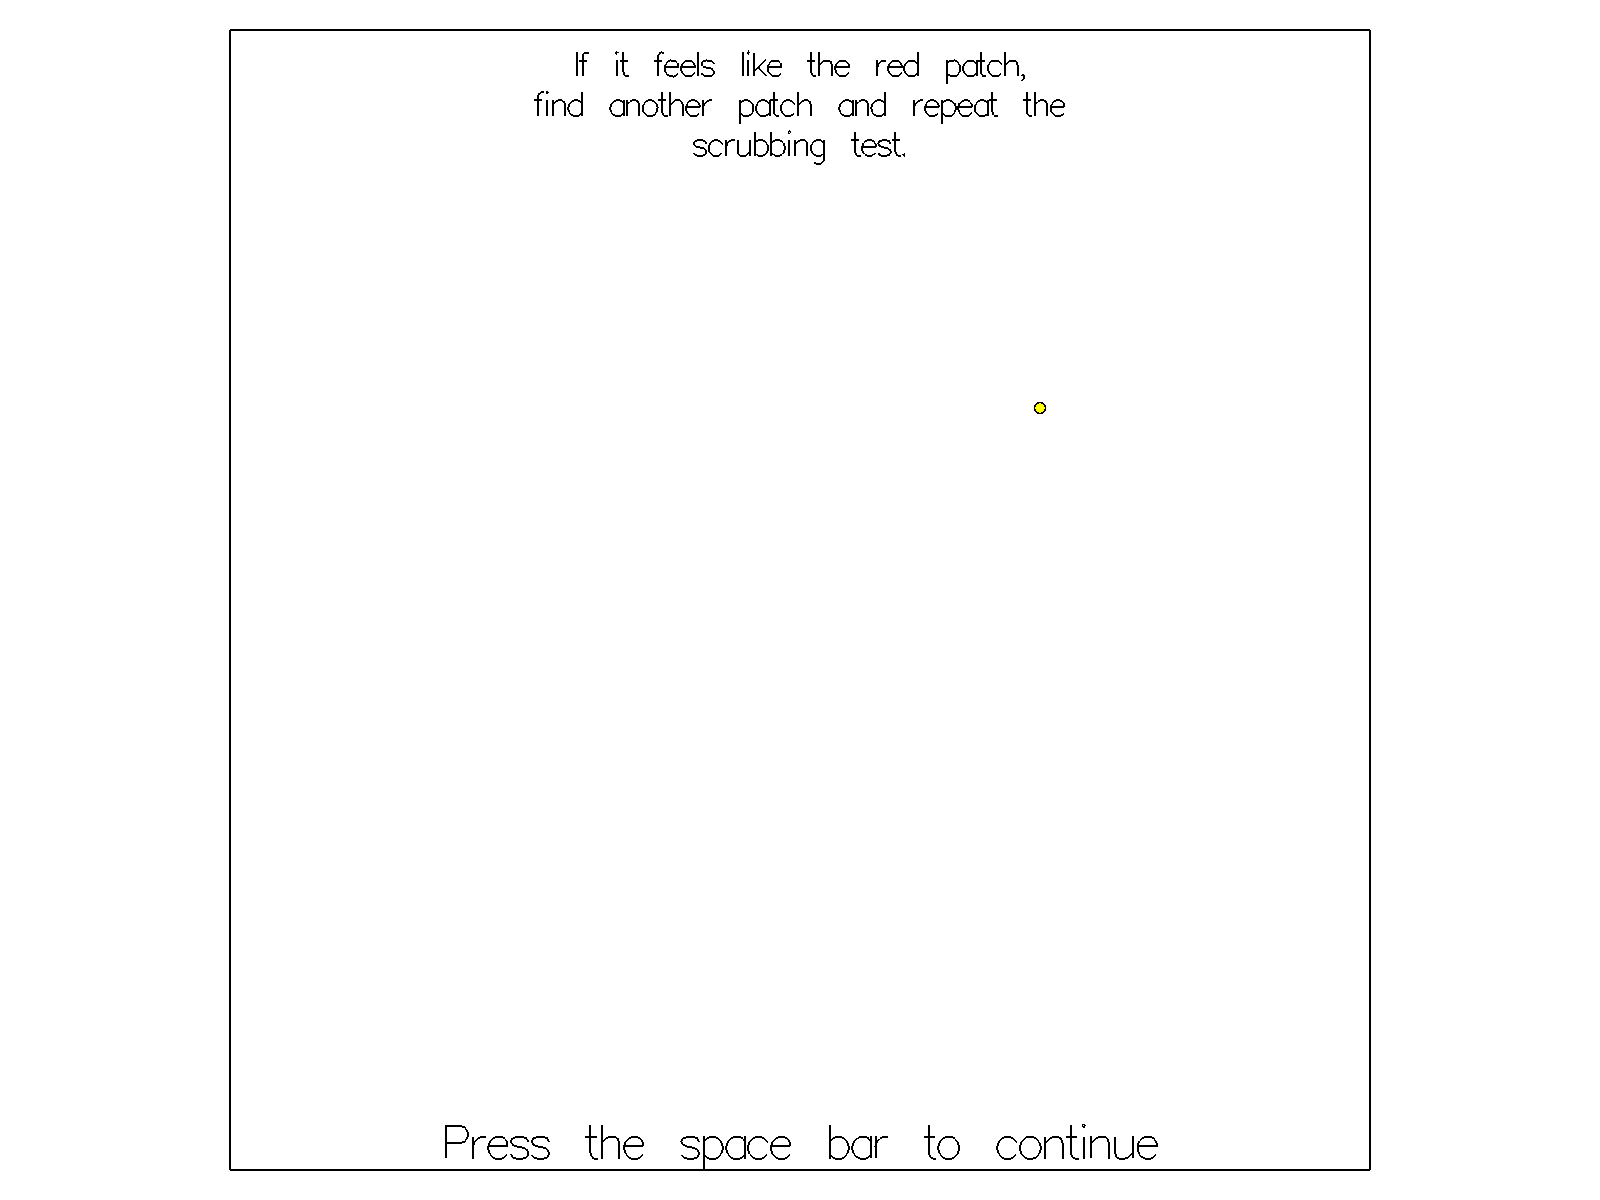
\includegraphics{figures/DecisionRed}}%
}%
\caption[]{}%
\label{fig:instructions10}%
\end{figure}%

\begin{figure}%
\ContinuedFloat%
\centering%
\subfloat[][]{%
\label{subfig:instructionsDecisionBlue}%
\fbox{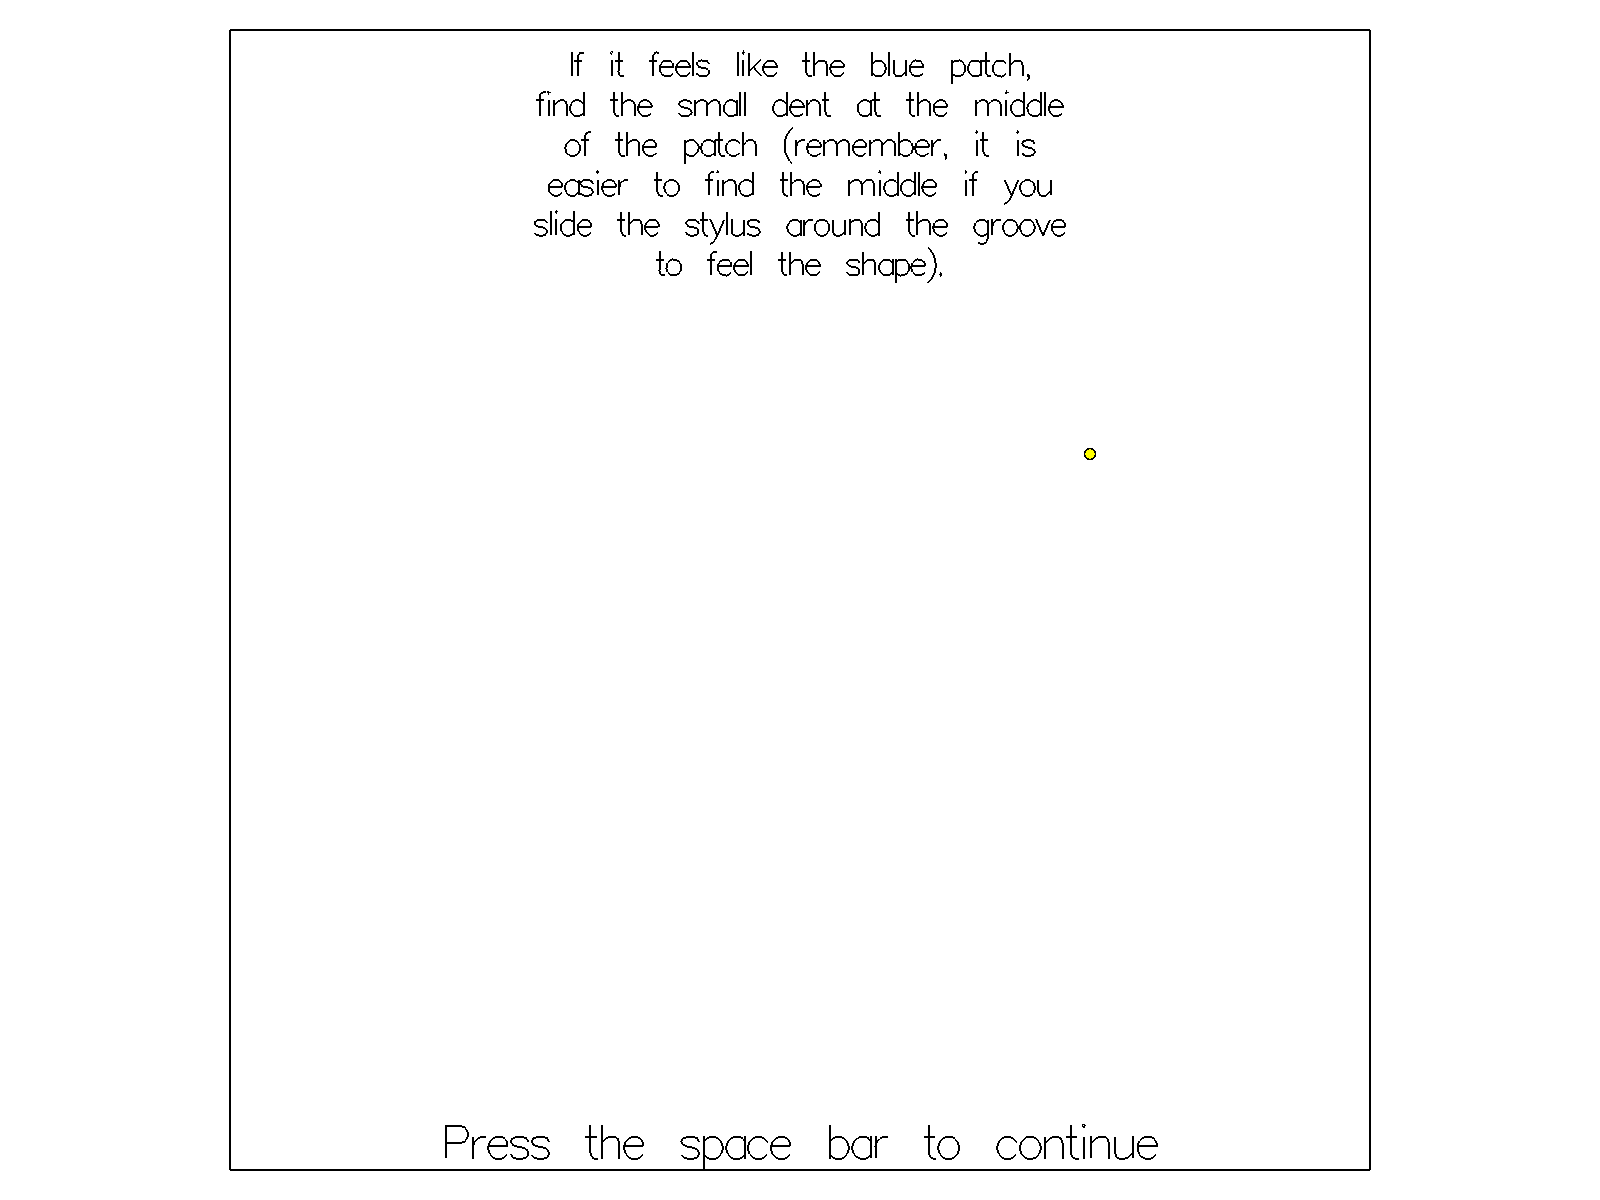
\includegraphics{figures/DecisionBlue}}%
}%
\linebreak%
\subfloat[][]{%
\label{subfig:instructionsEpisodeEnds}%
\fbox{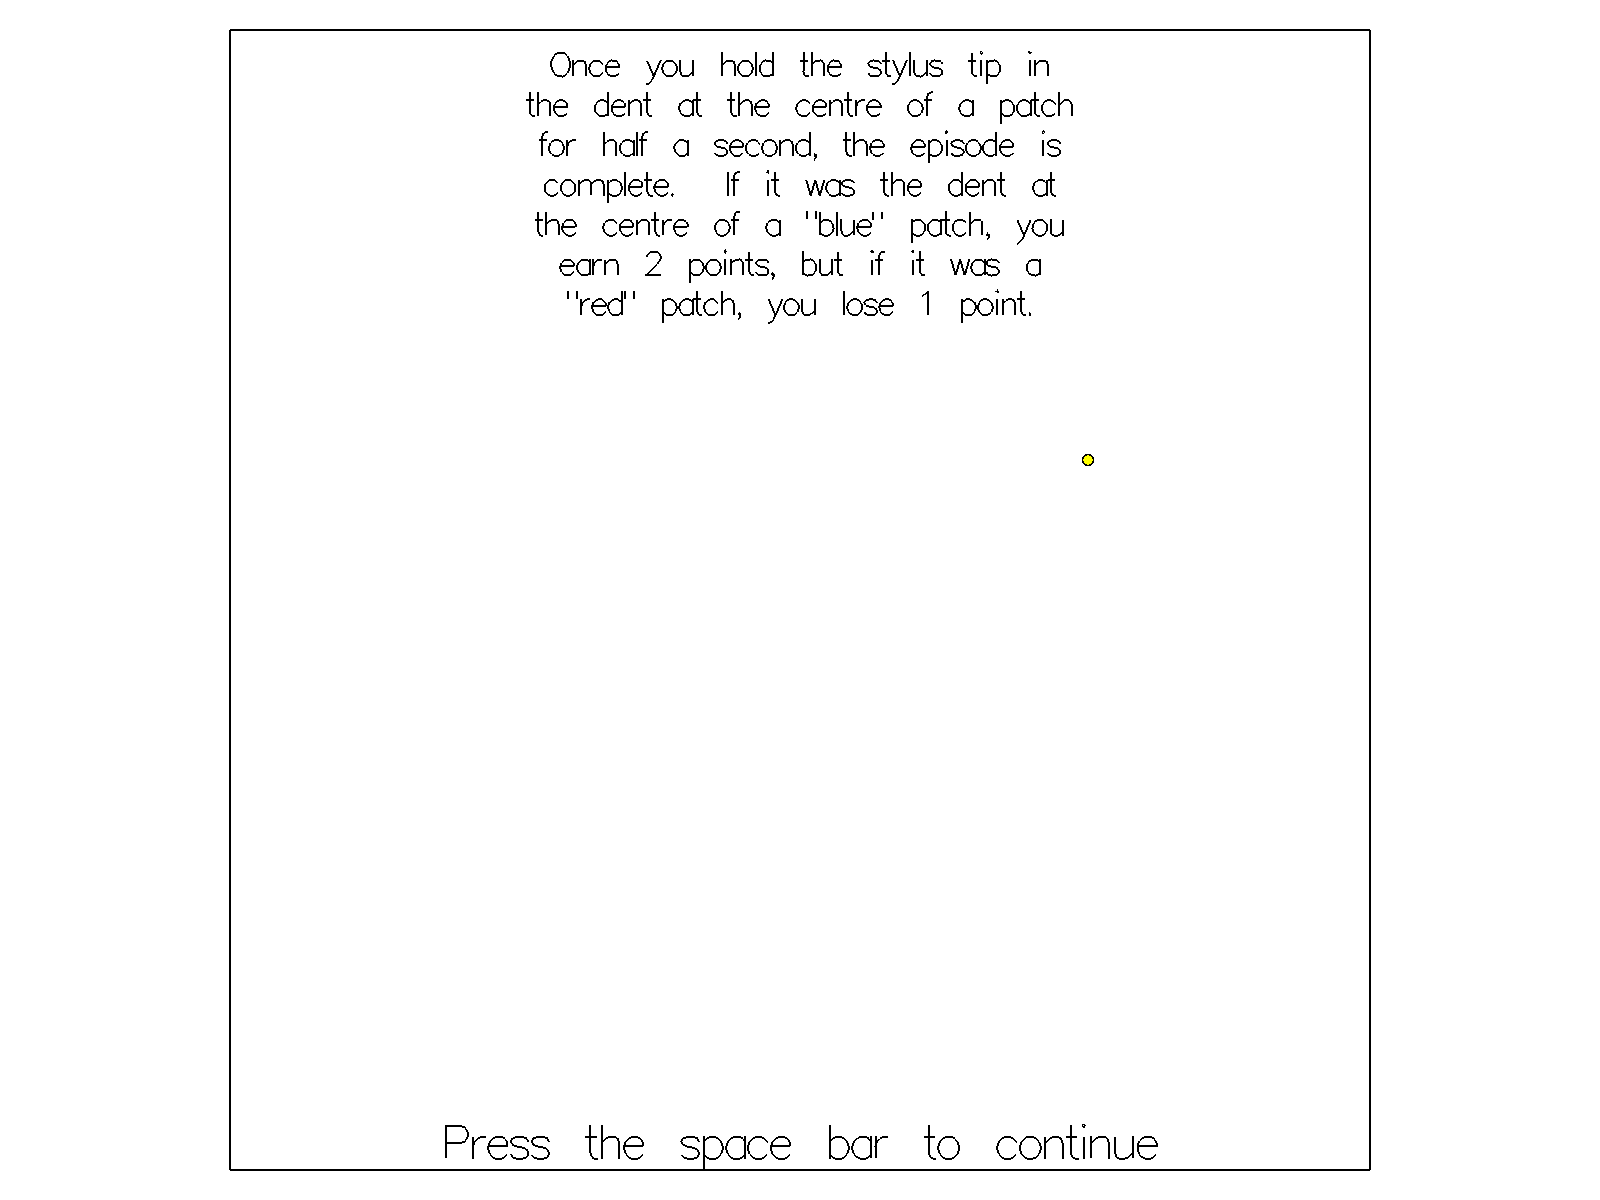
\includegraphics{figures/EpisodeEnds}}%
}%
\caption[]{}%
\label{fig:instructions11}%
\end{figure}%

\begin{figure}%
\ContinuedFloat%
\centering%
\subfloat[][If the subject selects the wrong (red) patch, the next screen is \subref{subfig:instructionsExampleFailure}; otherwise the next screen is \subref{subfig:instructionsExampleSuccess}.]{%
\label{subfig:instructionsTryExample}%
\fbox{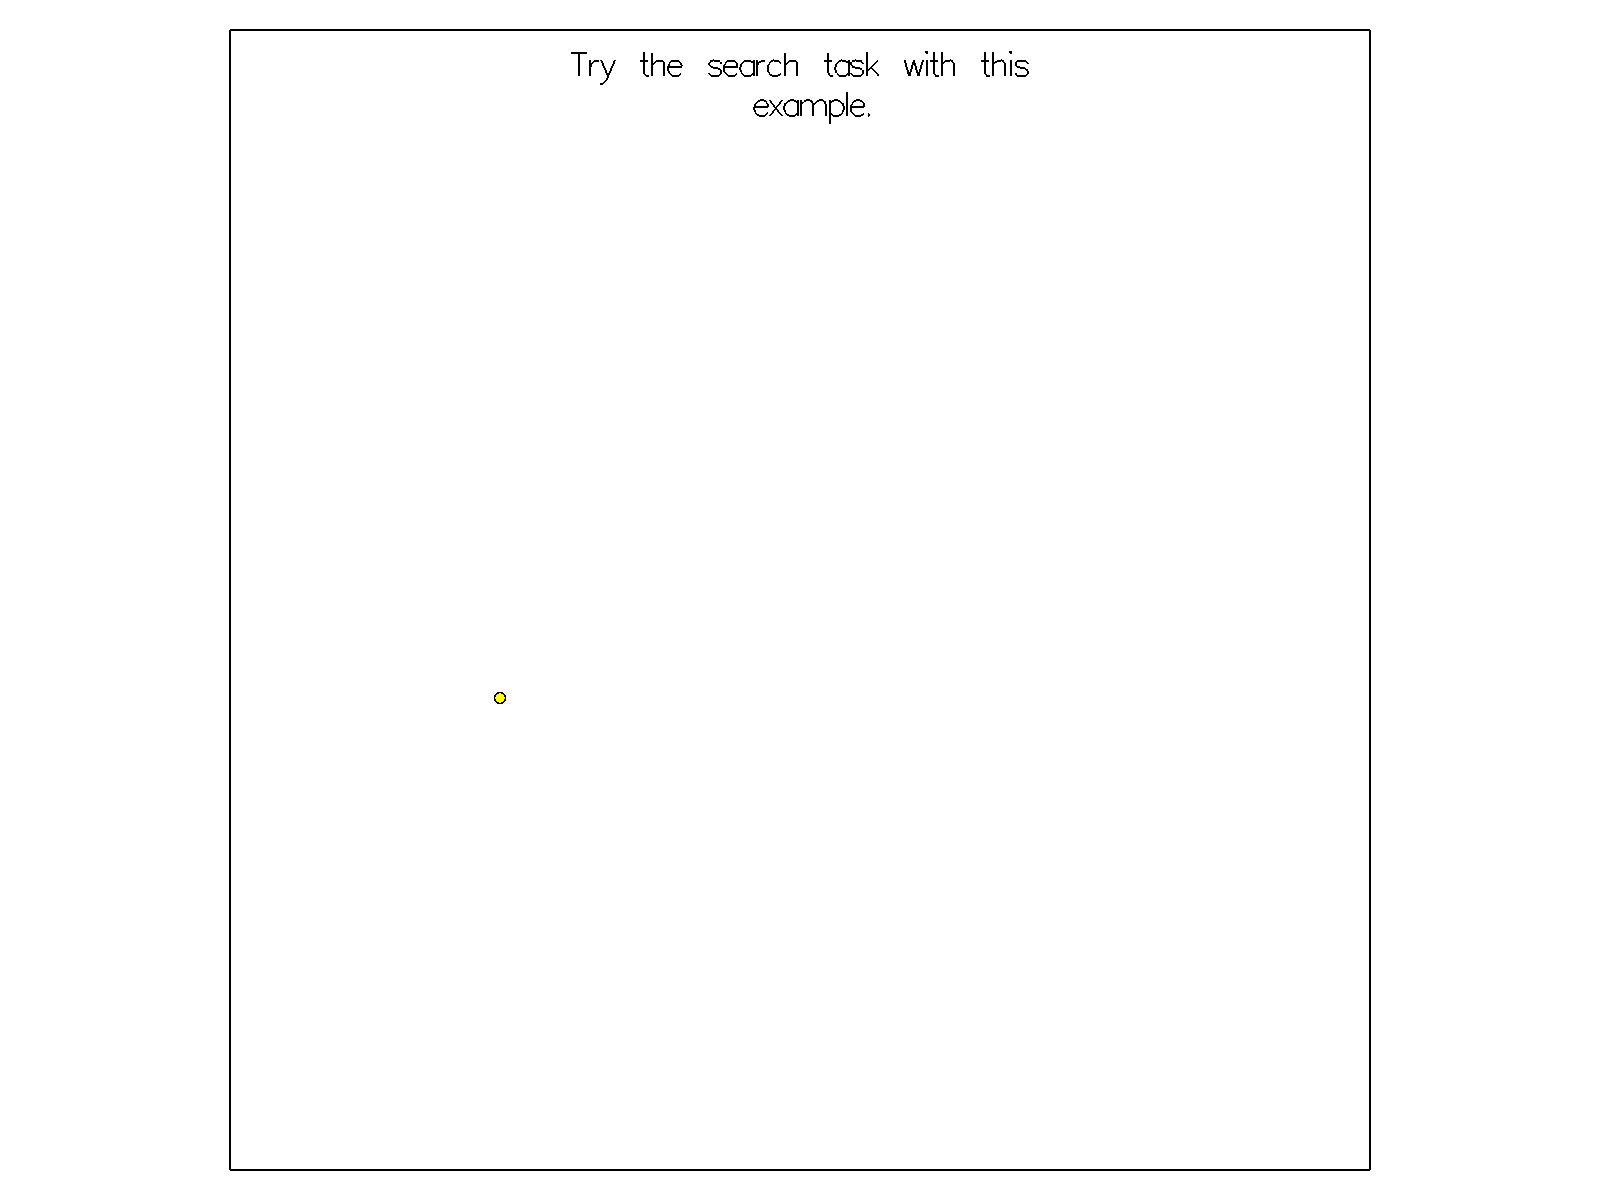
\includegraphics{figures/TryExample}}%
}%
\linebreak%
\subfloat[][After this screen, the subject is taken back to \subref{subfig:instructionsTryExample}.]{%
\label{subfig:instructionsExampleFailure}%
\fbox{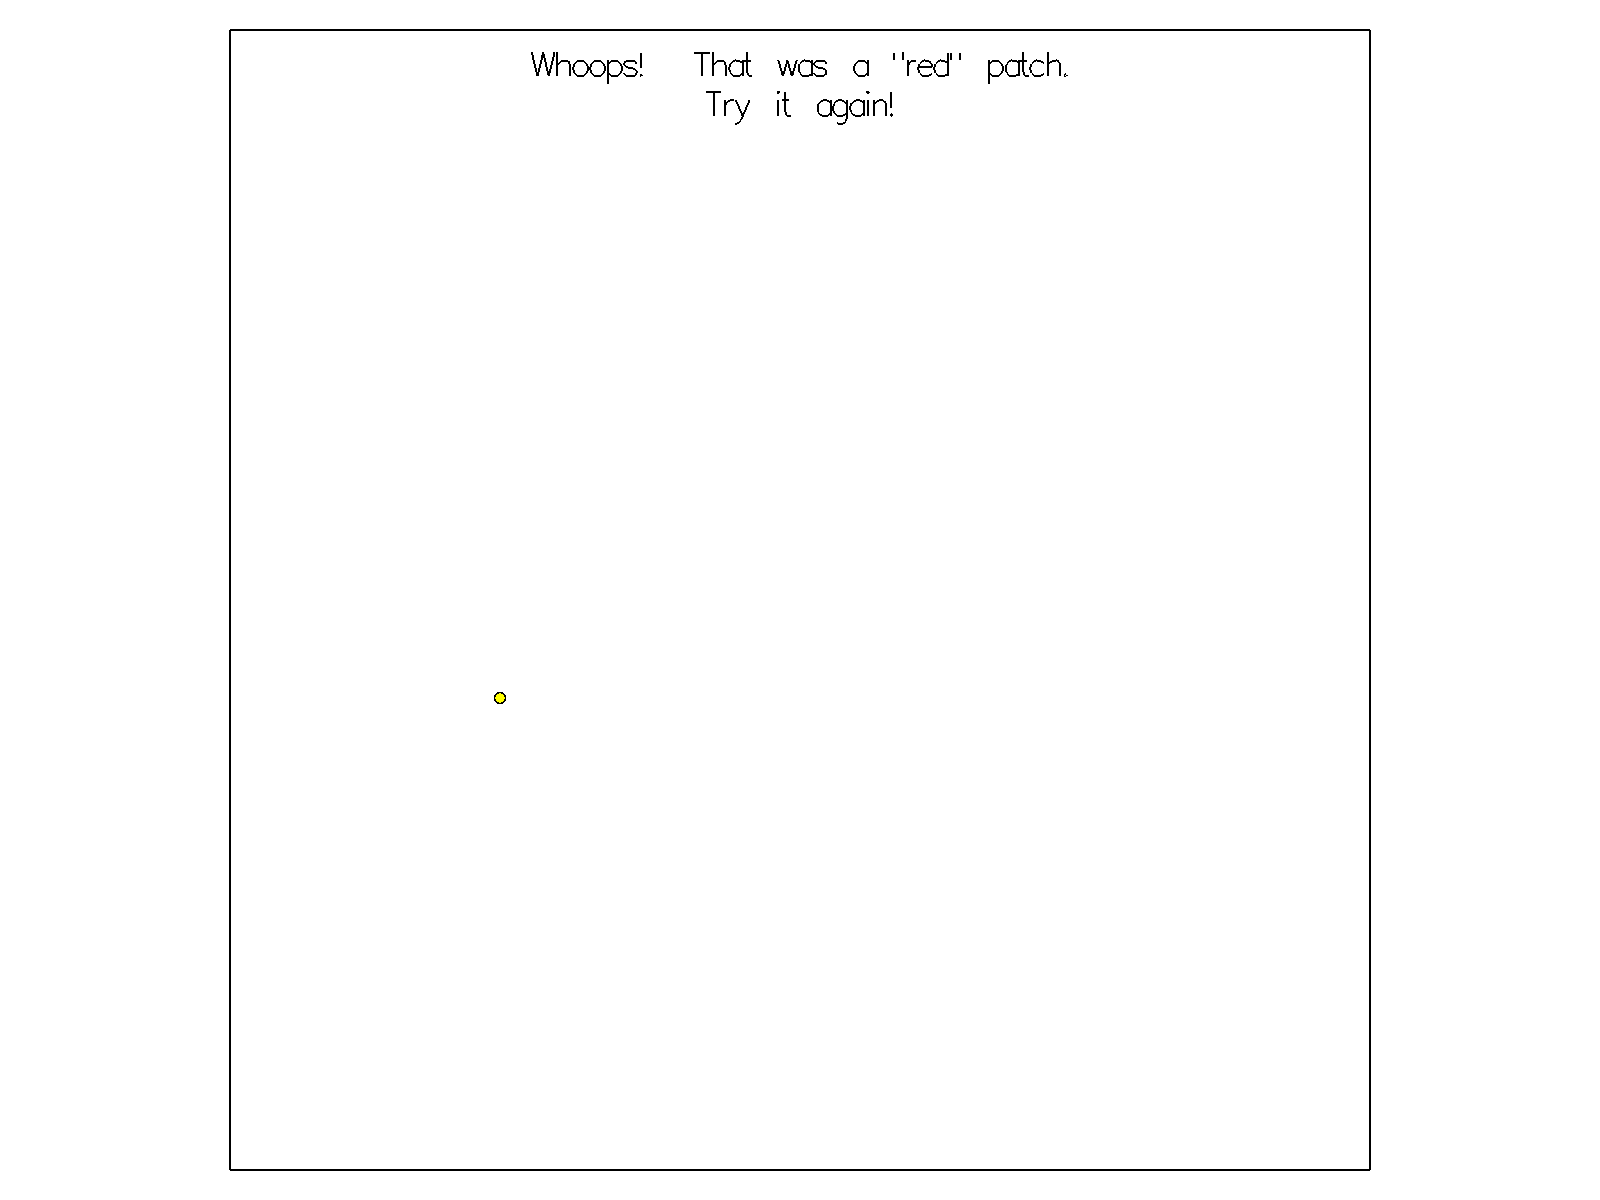
\includegraphics{figures/ExampleFailure}}%
}%
\caption[]{}%
\label{fig:instructions12}%
\end{figure}%

\begin{figure}%
\ContinuedFloat%
\centering%
\subfloat[][]{%
\label{subfig:instructionsExampleSuccess}%
\fbox{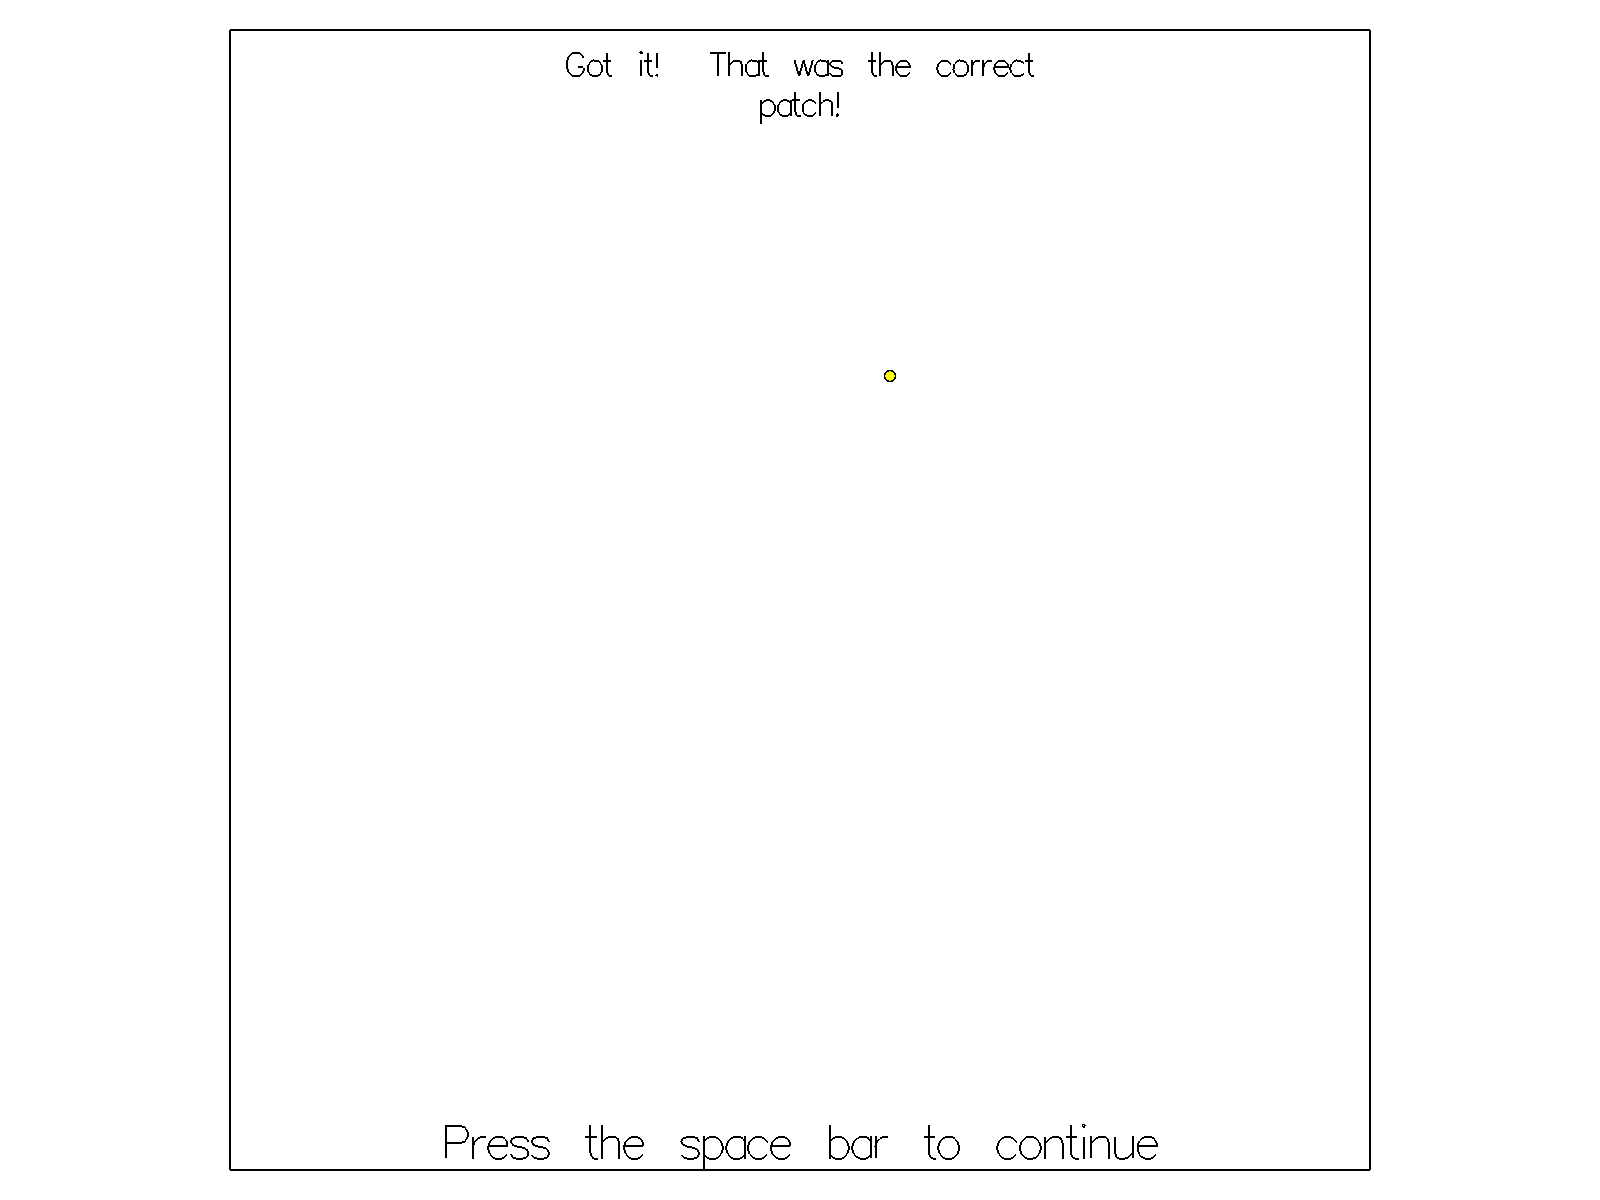
\includegraphics{figures/ExampleSuccess}}%
}%
\linebreak%
\subfloat[][]{%
\label{subfig:instructionsReadyToStartBaseline}%
\fbox{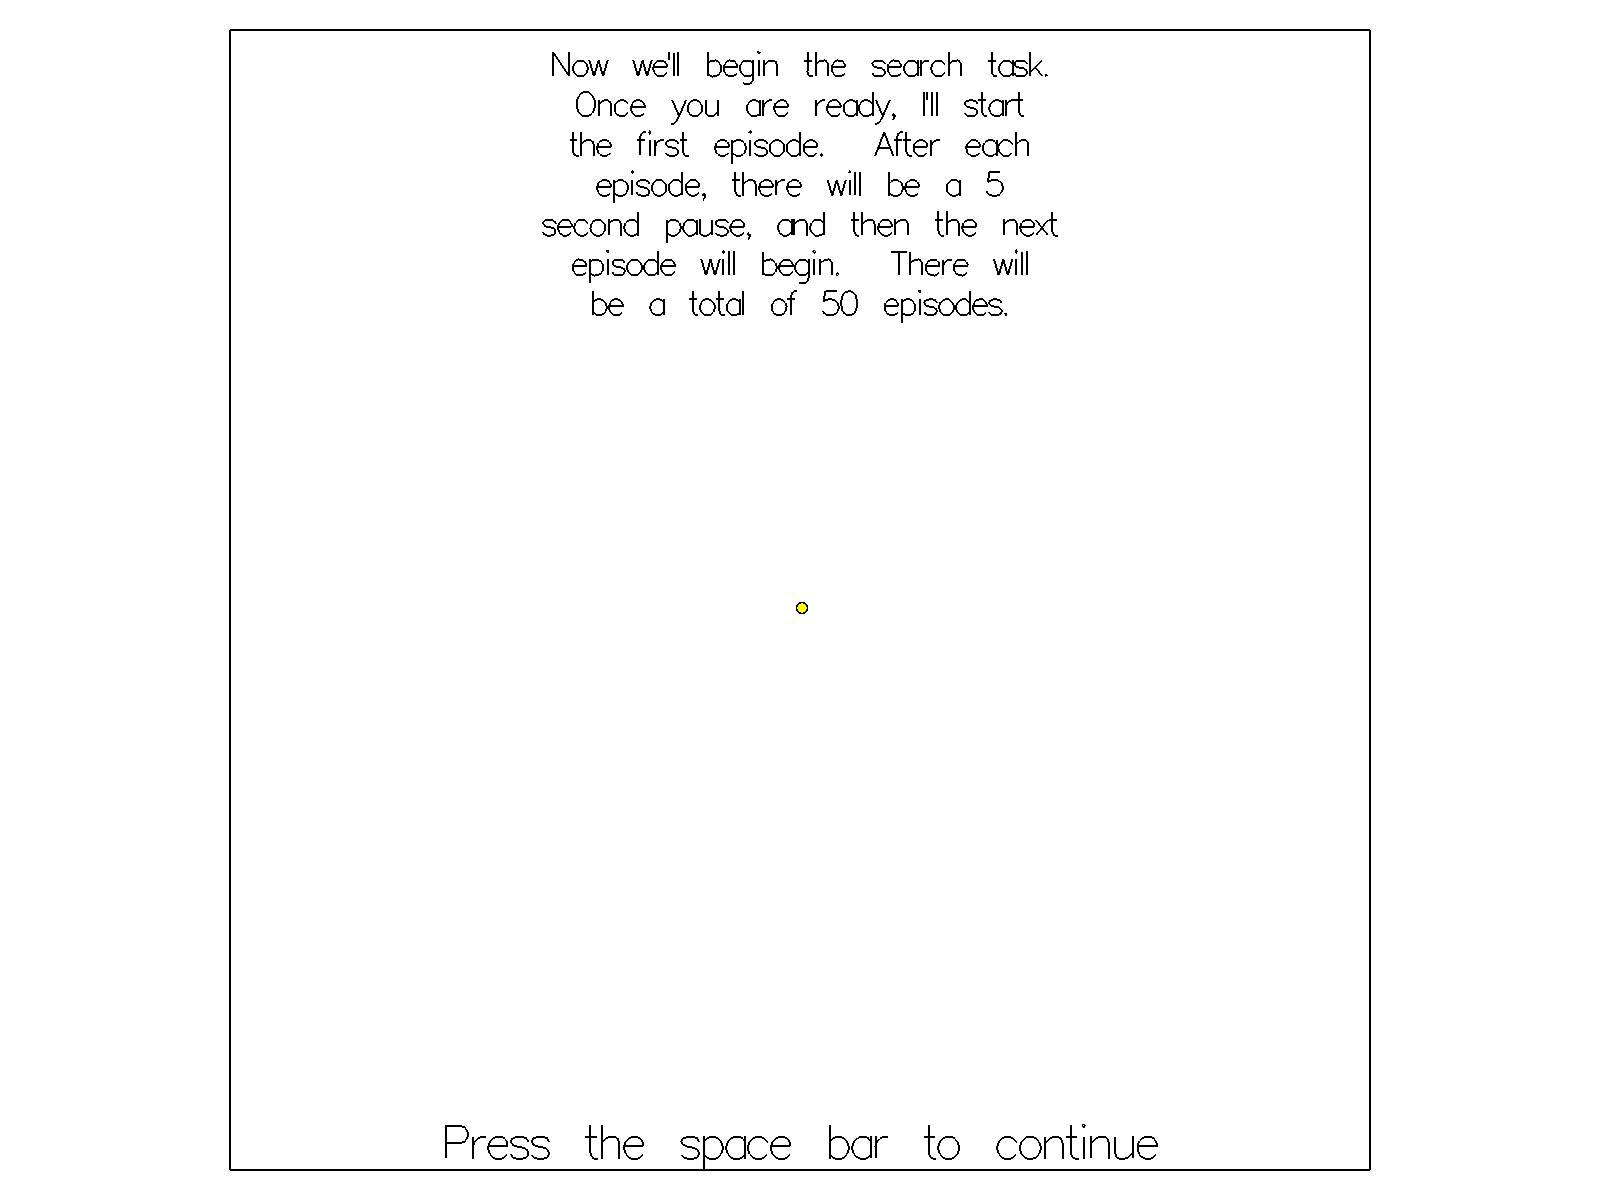
\includegraphics{figures/ReadyToStartBaseline}}%
}%
\caption[]{}%
\label{fig:instructions13}%
\end{figure}%
